%----------------------------------------------------------------------------------------
%    PACKAGES AND THEMES
%----------------------------------------------------------------------------------------

\documentclass[aspectratio=169,xcolor=dvipsnames]{beamer}
\usetheme{SimplePlus}

\usepackage{hyperref}
\usepackage{tikz}
\usepackage{graphicx}
\usepackage{transparent}
\usepackage{background}
\usepackage{booktabs} % Allows the use of \toprule, \midrule and \bottomrule in tables
\usepackage{subcaption}
\usepackage[style=authoryear,backend=biber]{biblatex}
\addbibresource{reference.bib} % Your .bib file


%----------------------------------------------------------------------------------------
%    TITLE PAGE
%----------------------------------------------------------------------------------------

\title{Graph Neural Networks in Computer Vision}
\subtitle{Hands-on Workshop on Deep Learning for Computer Vision \\ MG University}

\author{Ramzan Basheer}

\institute
{
    Research Scholar, Department of Avionics \\
    Indian Institute of Space Science and Technology - Thiruvananthapuram % Your institution for the title page
}
\date{\today} % Date, can be changed to a custom date

%----------------------------------------------------------------------------------------
%    PRESENTATION SLIDES
%----------------------------------------------------------------------------------------

\begin{document}

\begin{frame}
    % Print the title page as the first slide
    \titlepage
\end{frame}

\begin{frame}{Overview}
    % Throughout your presentation, if you choose to use \section{} and \subsection{} commands, these will automatically be printed on this slide as an overview of your presentation
    \tableofcontents
\end{frame}

%------------------------------------------------
\section{Introduction}
%------------------------------------------------

\begin{frame}{Traditional Neural Networks}
    \begin{tikzpicture}[remember picture, overlay]
        \node at (9.3,1) {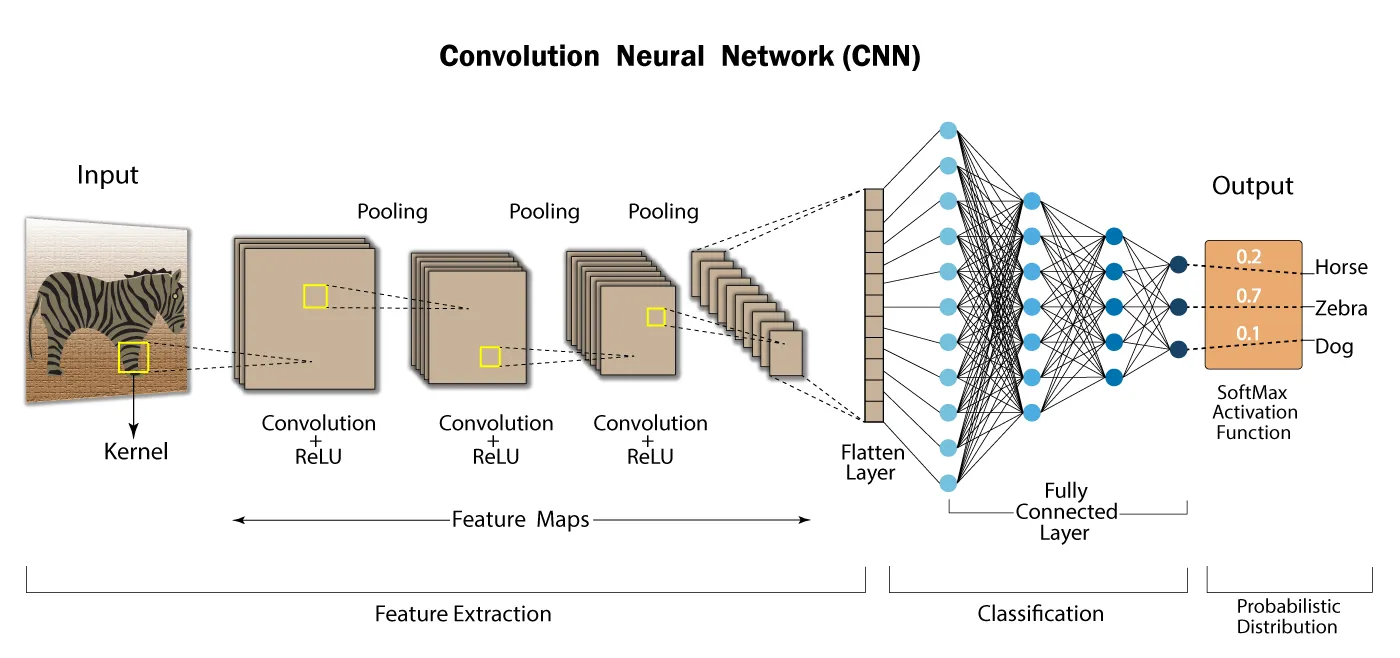
\includegraphics[width=0.7\textwidth,height=0.4\textheight, keepaspectratio]{figures/s1/lenet.png}};
    
         
    
        \node at (2,2) 
        {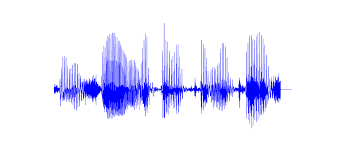
\includegraphics[width=0.3\textwidth,height=0.2\textheight, keepaspectratio]{figures/s1/audio.png}};
    
         
    
        \node at (2,-0.1) {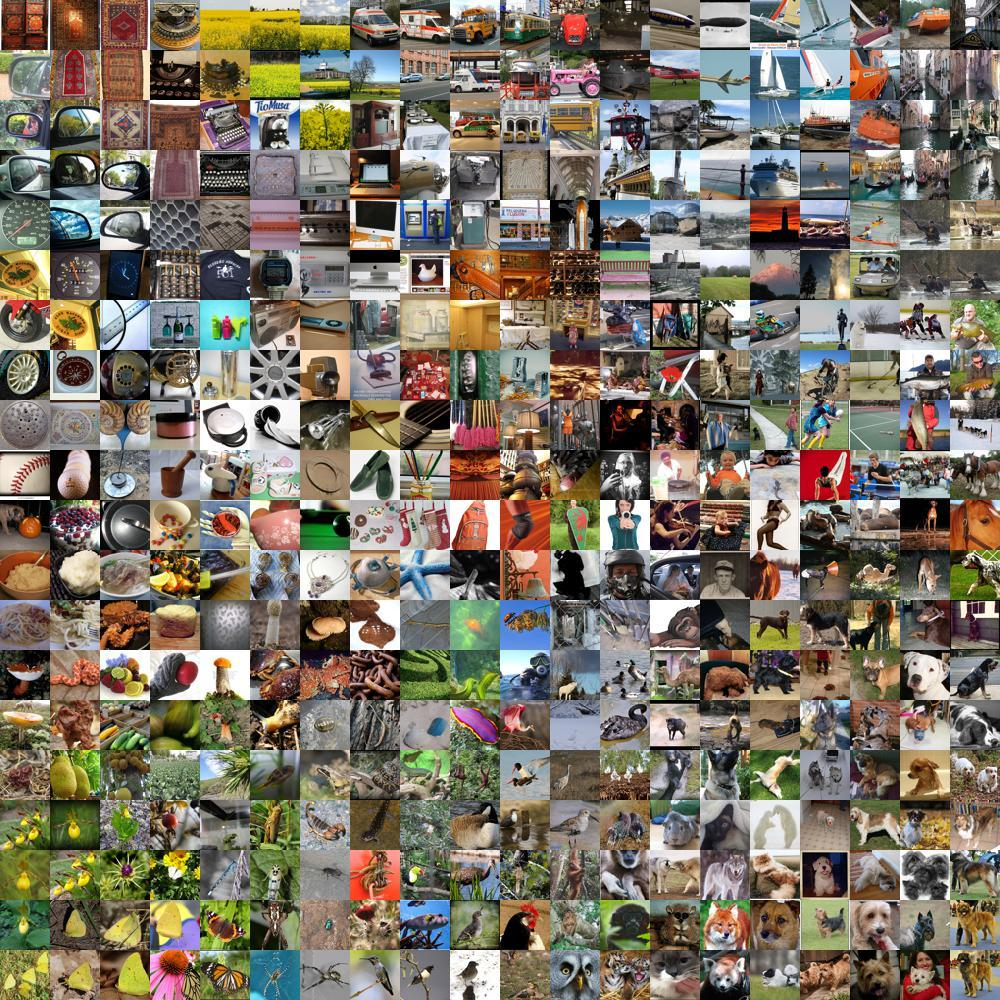
\includegraphics[width=0.4\textwidth,height=0.3\textheight, keepaspectratio]{figures/s1/images.jpg}};
    
         
    
        \node at (6.5,-1.2) {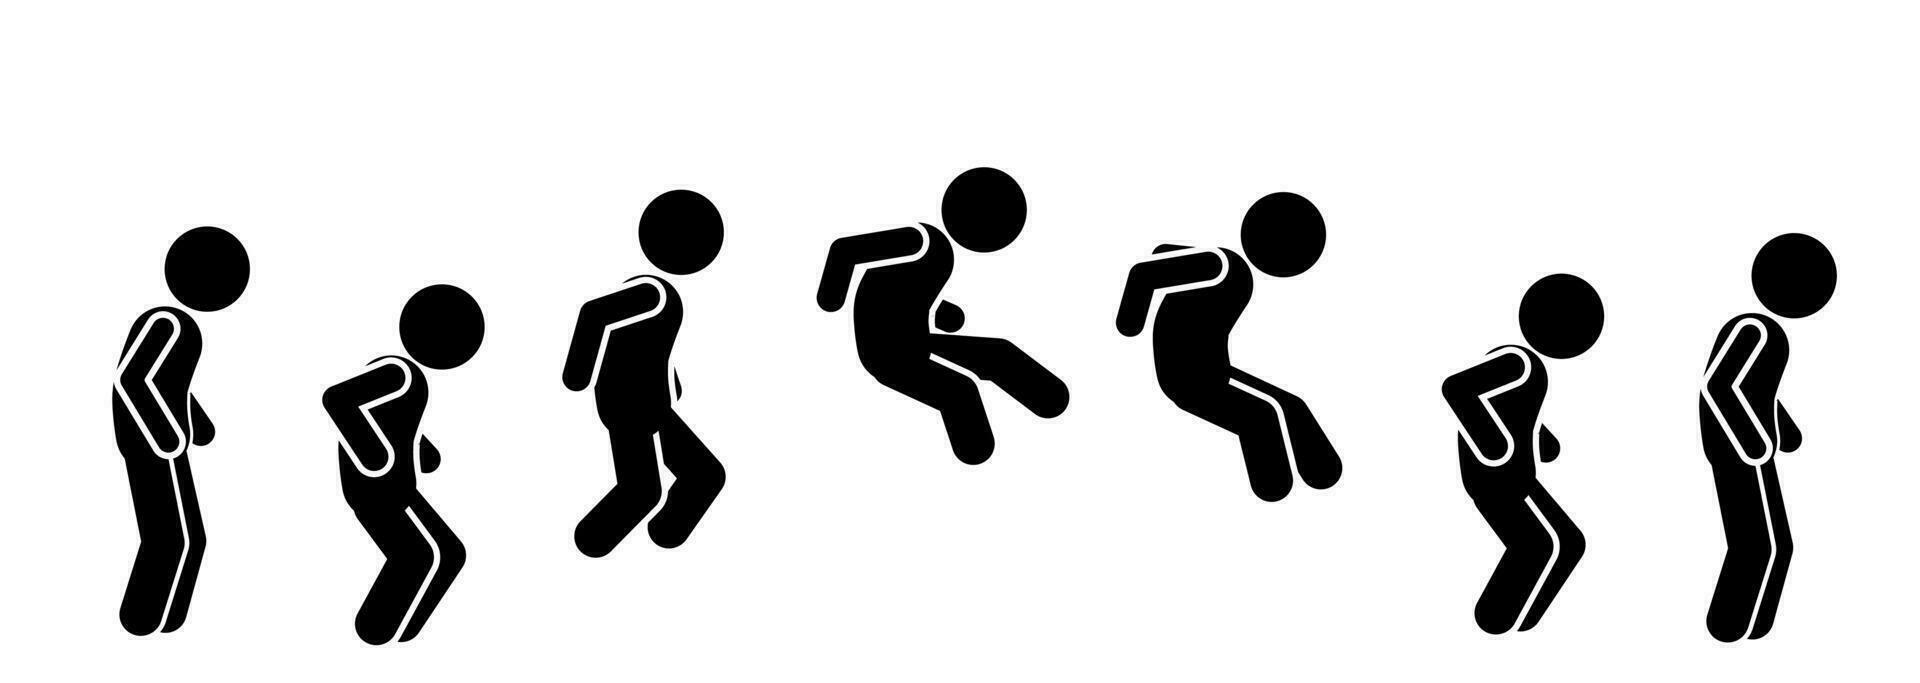
\includegraphics[width=0.4\textwidth,height=0.17\textheight, keepaspectratio]{figures/s1/video_seq.jpg}};
    
         
    
        \node at (11.5,-1.2) {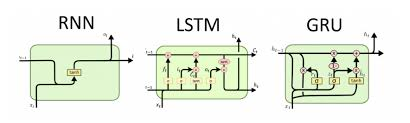
\includegraphics[width=0.35\textwidth,height=0.17\textheight, keepaspectratio]{figures/s1/RNN_LSTM_GRU.jpeg}};

        \node at (current page.south) [anchor=south, yshift=0.8cm, text width=0.9\textwidth] {
        Deep neural networks are designed for sequences and grids exploiting
        \begin{itemize}
            \item Translation equivariance (weight sharing)
            \item Hierarchical compositionality
        \end{itemize}
        };
    \end{tikzpicture}
\end{frame}

\begin{frame}{Real-world data are rarely on grids!}
    \begin{figure}
        \centering
        \begin{subfigure}{0.48\textwidth}
          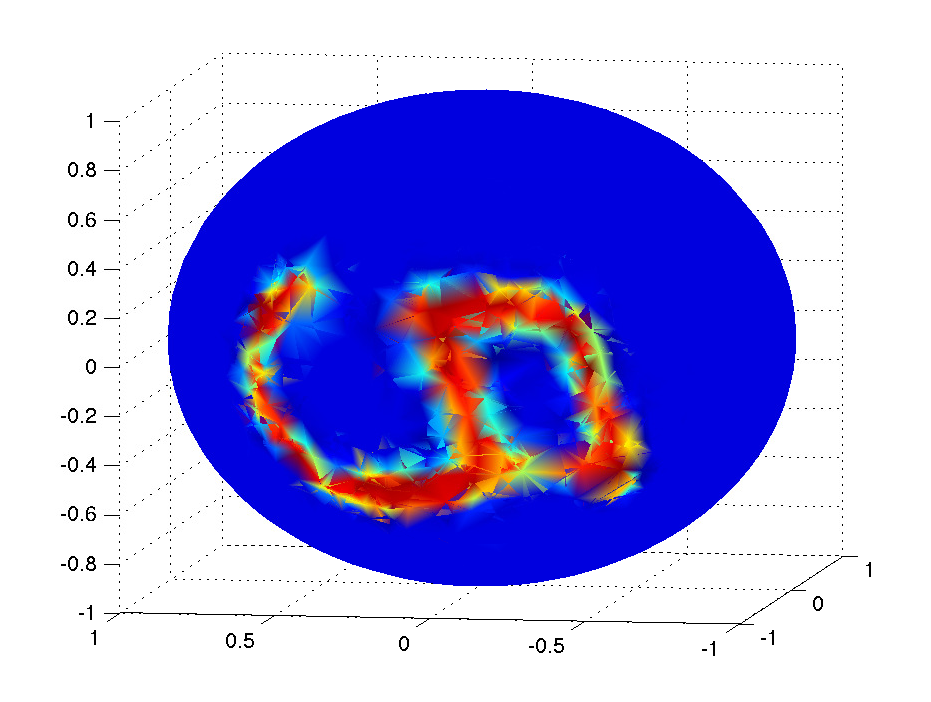
\includegraphics[width=\linewidth]{figures/sphere_ex1.pdf}
        \end{subfigure}
        \hfill
        \begin{subfigure}{0.48\textwidth}
          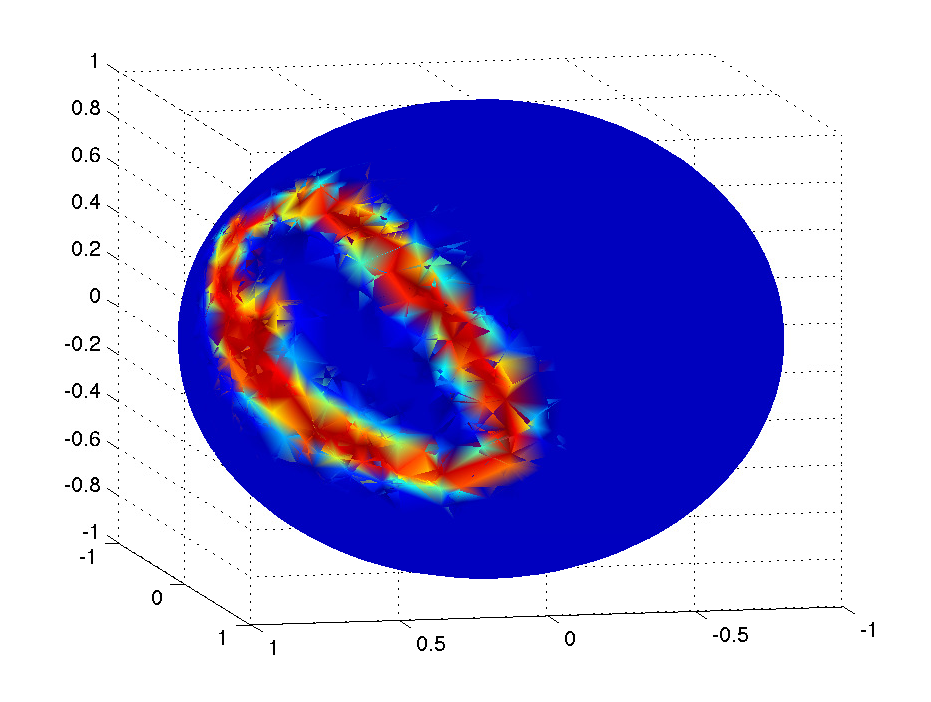
\includegraphics[width=\linewidth]{figures/sphere_ex2.pdf}
        \end{subfigure}
        \caption*{Examples of some MNIST digits on the sphere.\footfullcite{bruna2014spectral}}
  \end{figure}
\end{frame}

\begin{frame}{}
    \begin{tikzpicture}[remember picture, overlay]
            \node at (1.6,1.7) {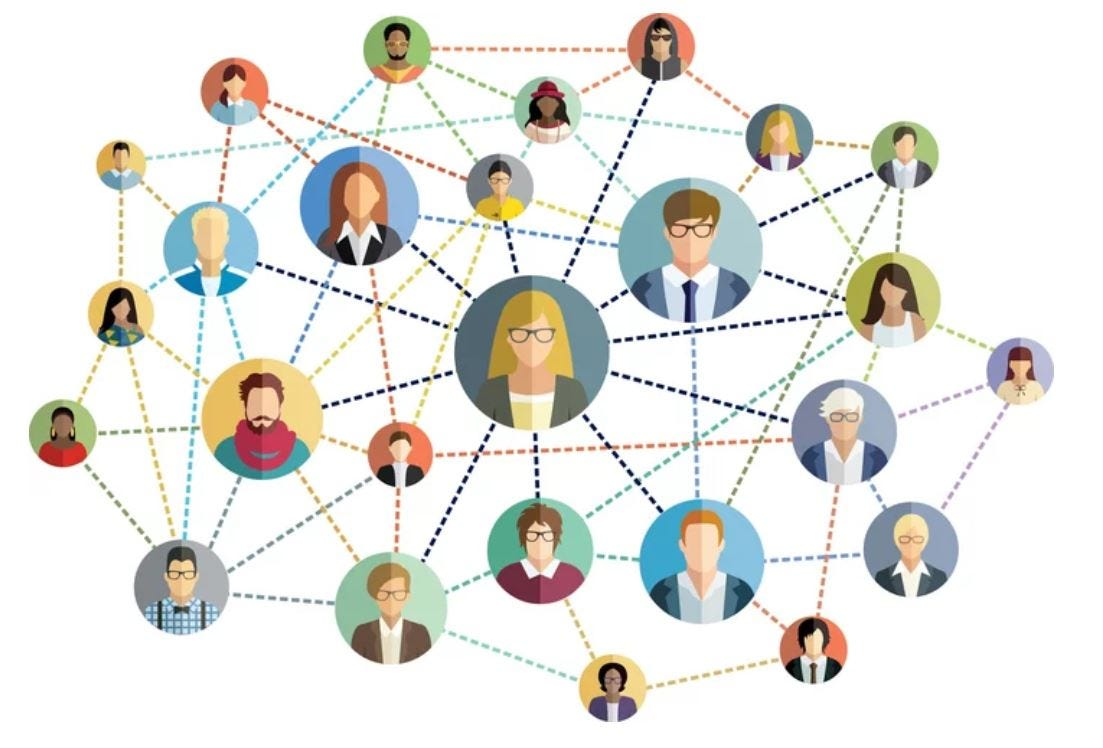
\includegraphics[width=0.3\textwidth,height=0.35\textheight, keepaspectratio]{figures/s2/social_network.jpg}};
            \node at (1.6,-0.3) {Social Networks};
        
            \node at (6.5,1.6)             {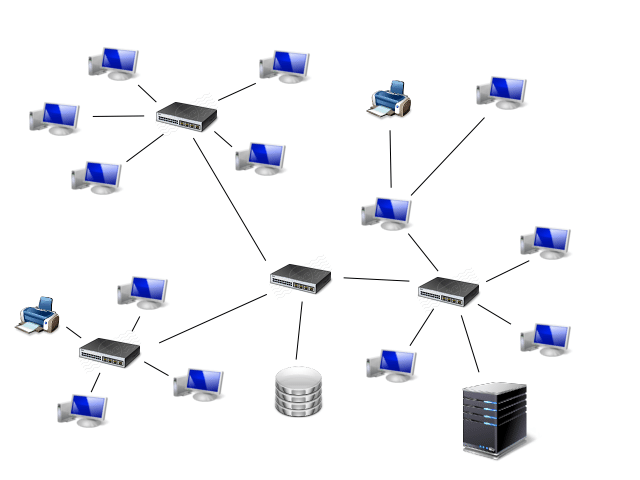
\includegraphics[width=0.4\textwidth,height=0.4\textheight, keepaspectratio]{figures/s2/A-computer-network.png}};
            \node at (6.5,-0.2){Computer Networks};
        
            \node at (3.5,-2) {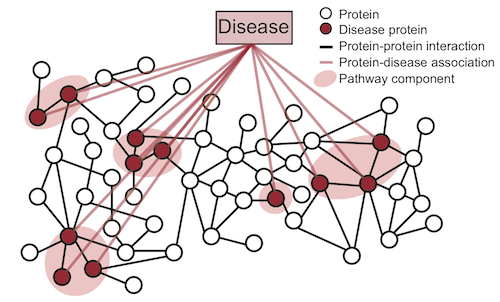
\includegraphics[width=0.4\textwidth,height=0.3\textheight, keepaspectratio]{figures/s2/disease-pathway.png}};
            \node at (3.5,-3.7){Disease Pathways};
        
            \node at (9.5,-2.5) {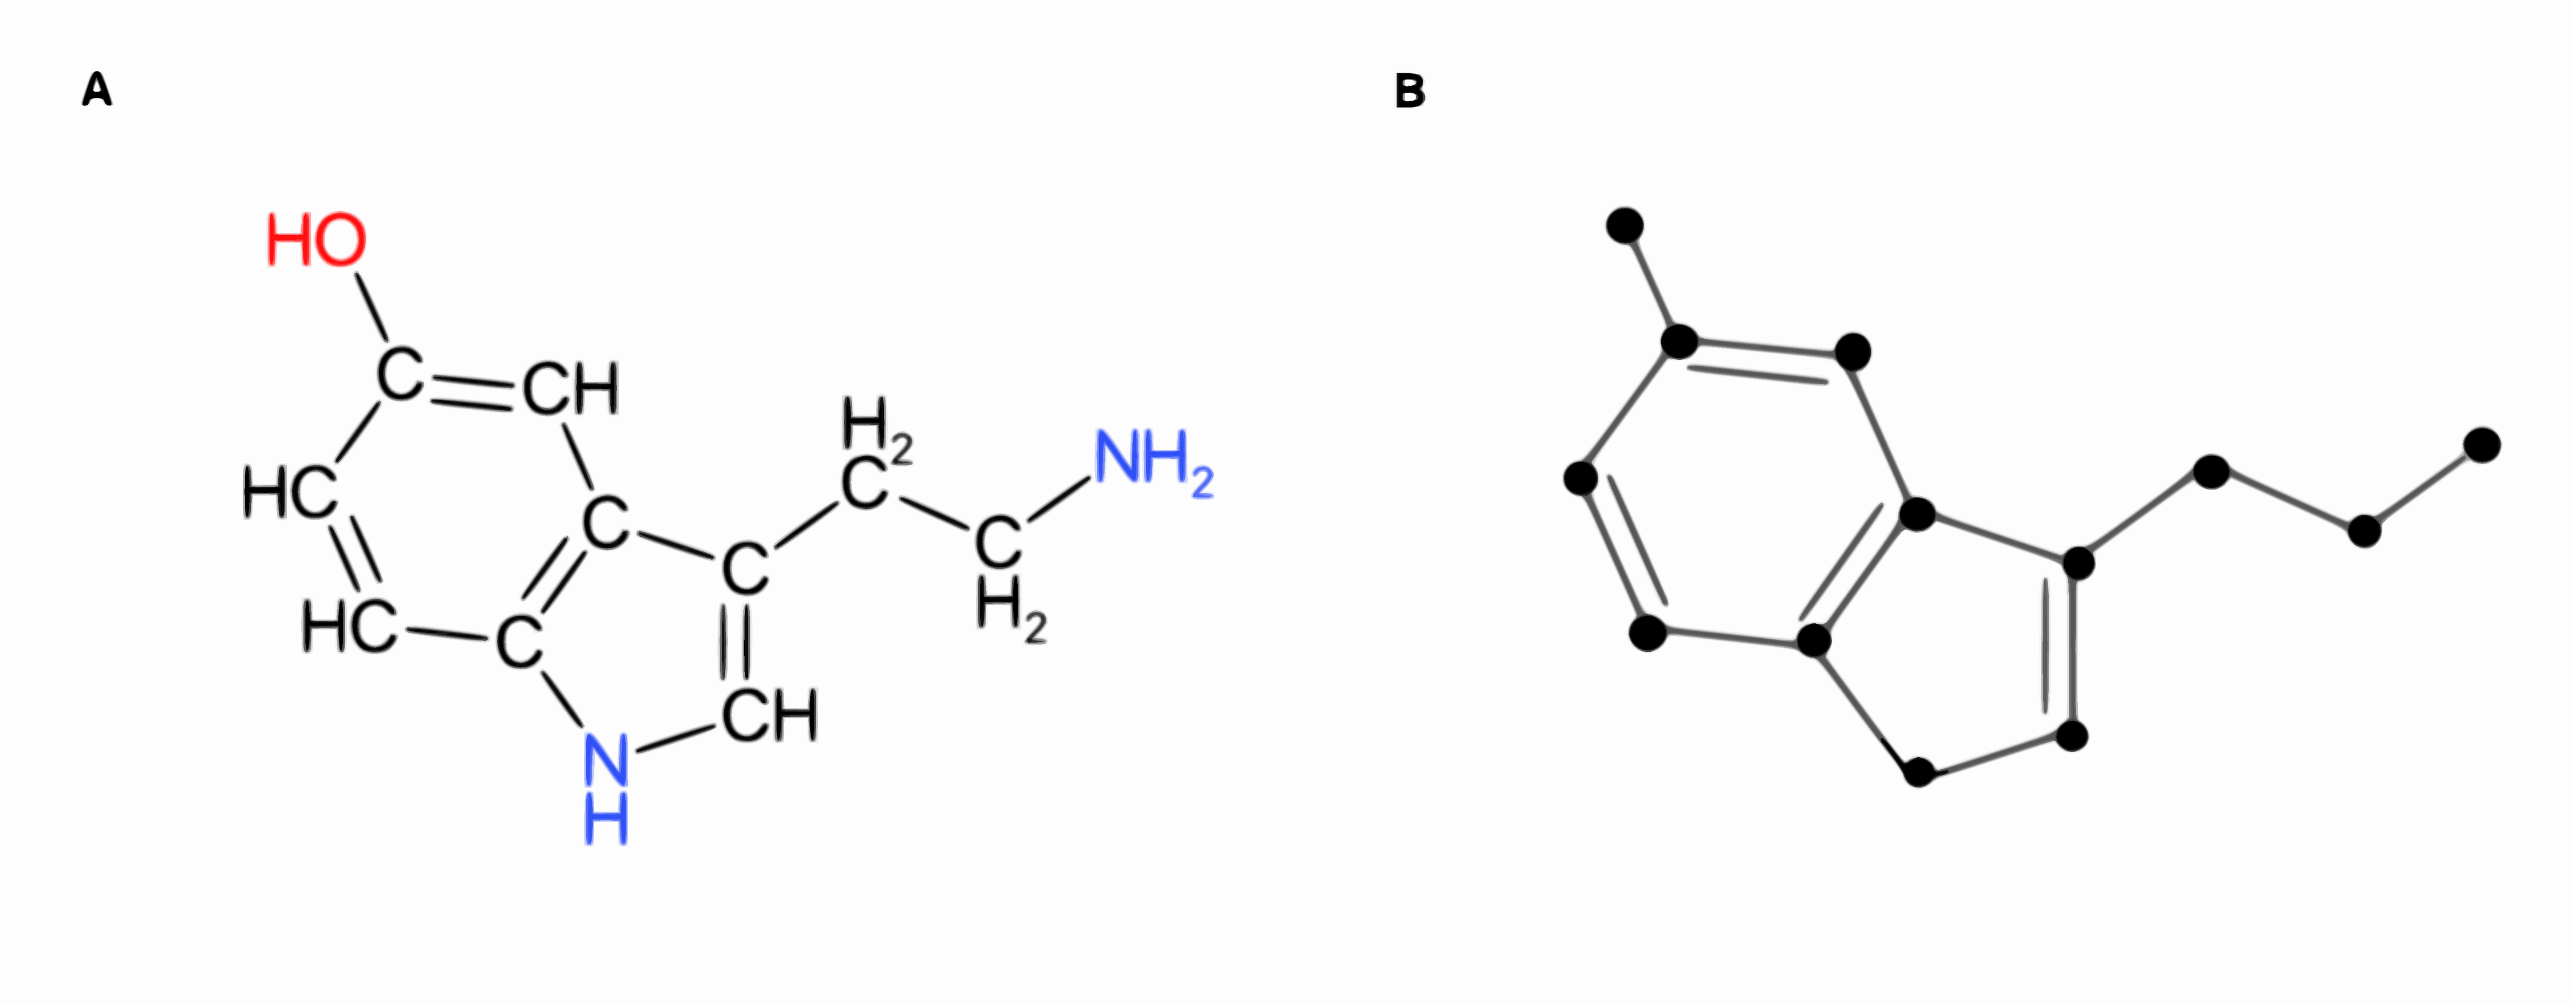
\includegraphics[width=0.4\textwidth,height=0.4\textheight, keepaspectratio]{figures/s2/molecularGraph.png}};
            \node at (9.5,-3.7){Molecular Graphs};
        
            \node at (11.5,1) {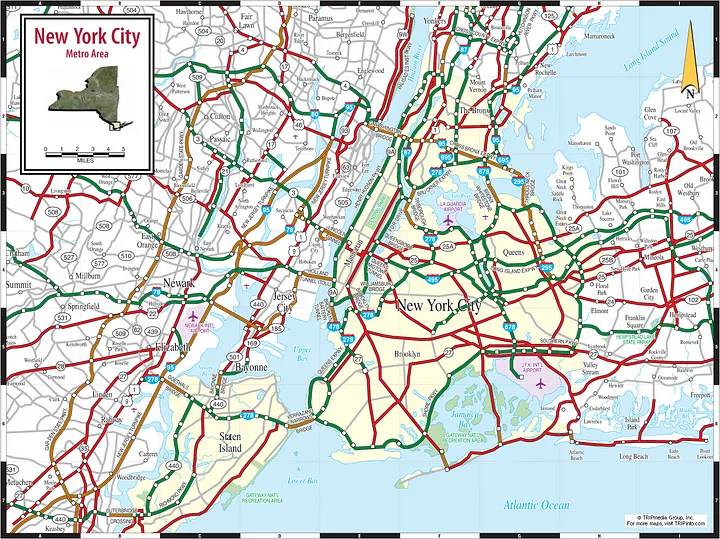
\includegraphics[width=0.4\textwidth,height=0.4\textheight, keepaspectratio]{figures/s2/nycmap.png}};
            \node at (11.5,-1){Transportation Networks};
        \end{tikzpicture}
\end{frame}

\begin{frame}{}
    \begin{tikzpicture}[remember picture, overlay]
        \node at (1.6,1.7) {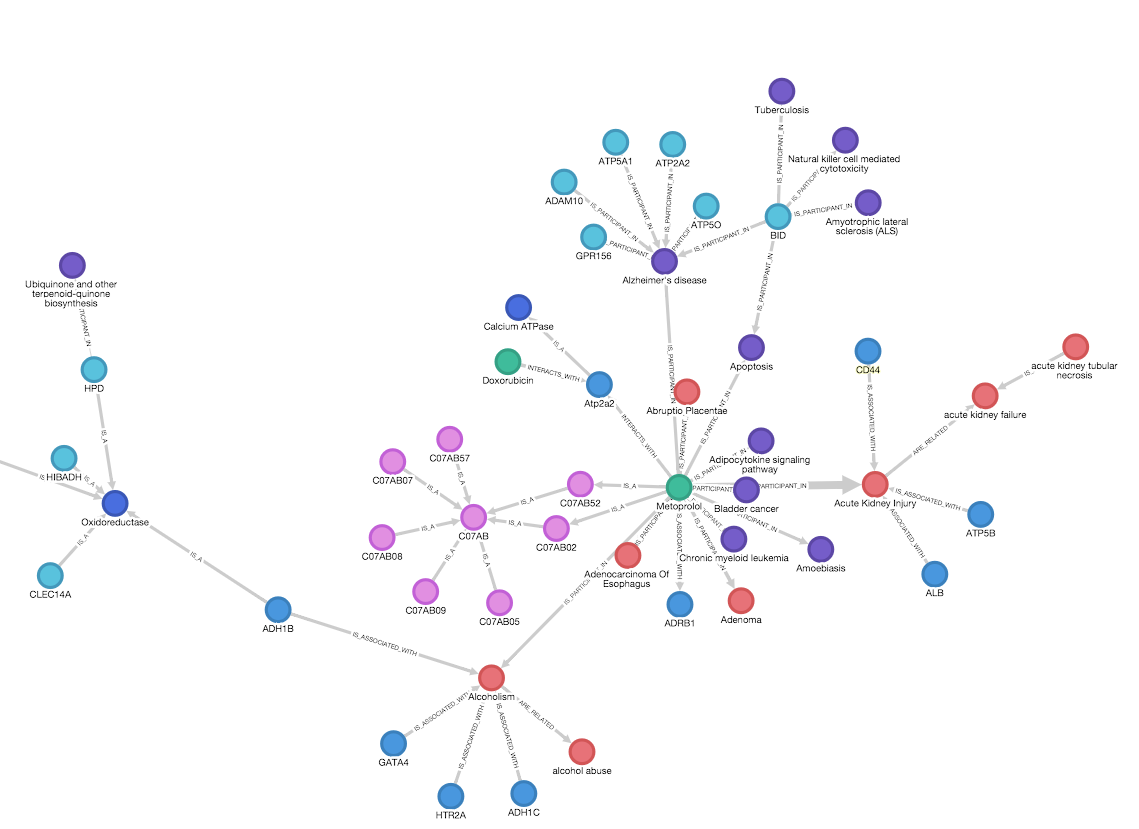
\includegraphics[width=0.3\textwidth,height=0.3\textheight, keepaspectratio]{figures/s2/knowledge_graphs.png}};
        \node at (1.6,-0.22) {Knowledge Graphs};
    
        \node at (6.5,1.5)             {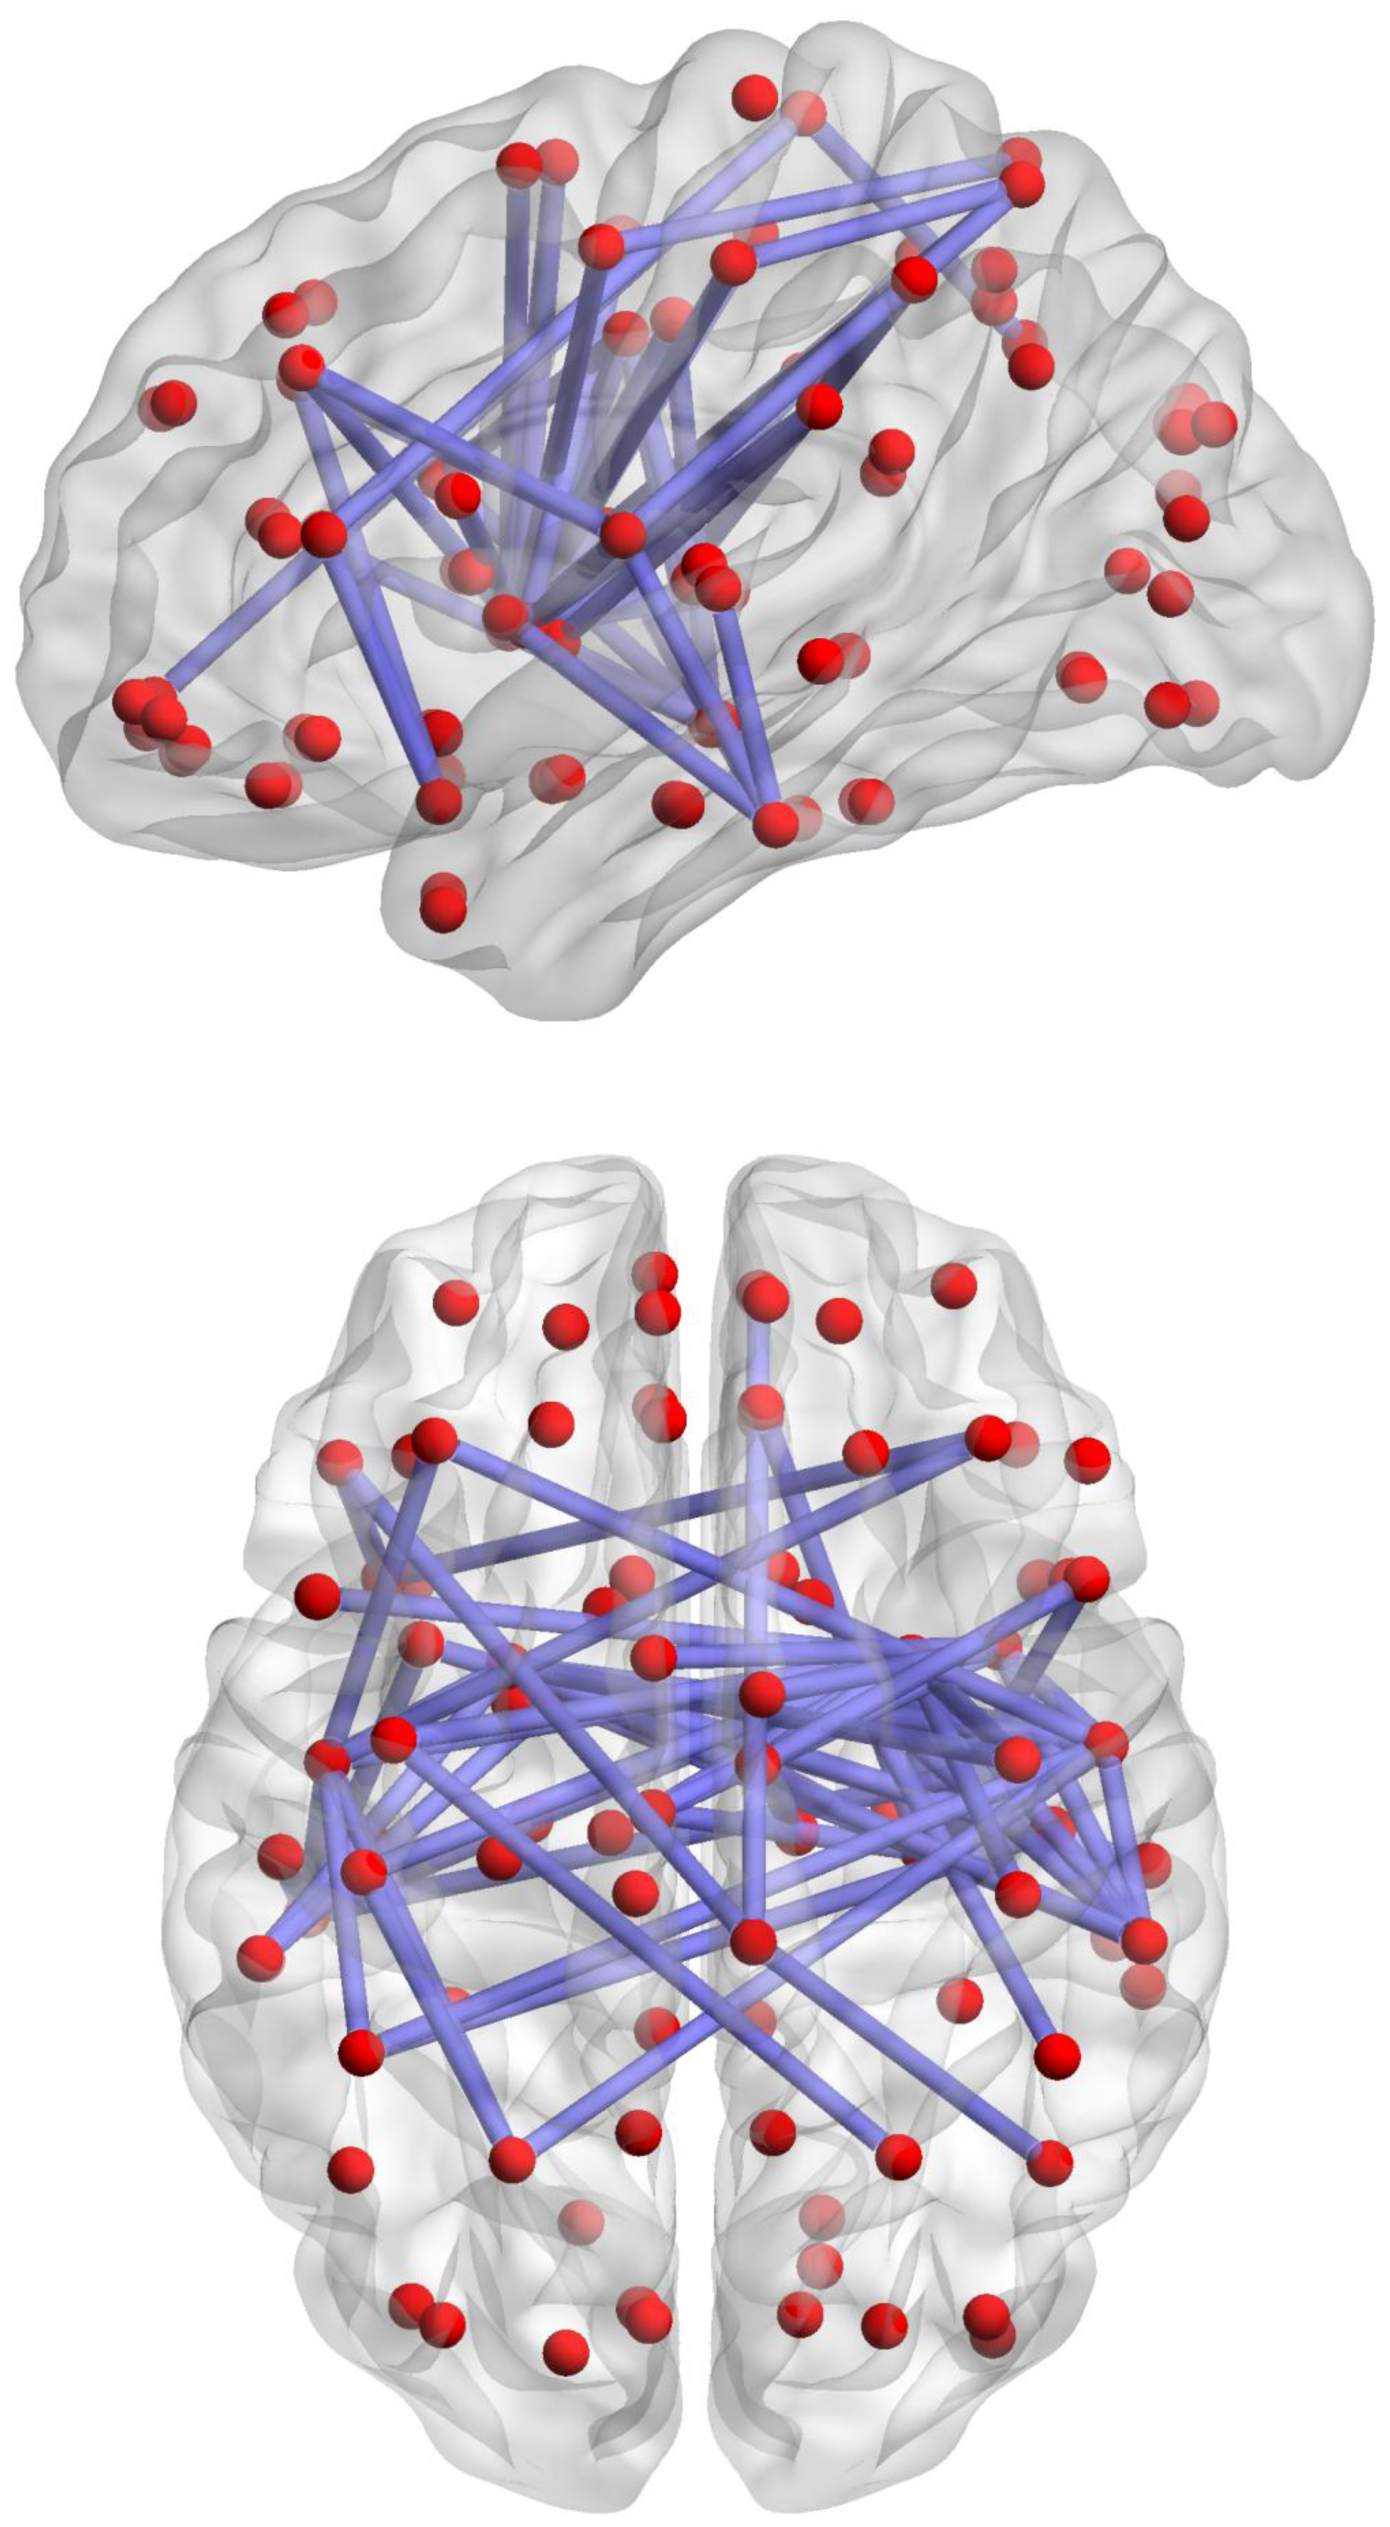
\includegraphics[width=0.4\textwidth,height=0.4\textheight, keepaspectratio]{figures/s2/Brain_network.png}};
        \node at (6.5,-0.5){Brain Networks};  
    
        \node at (2.5,-2) {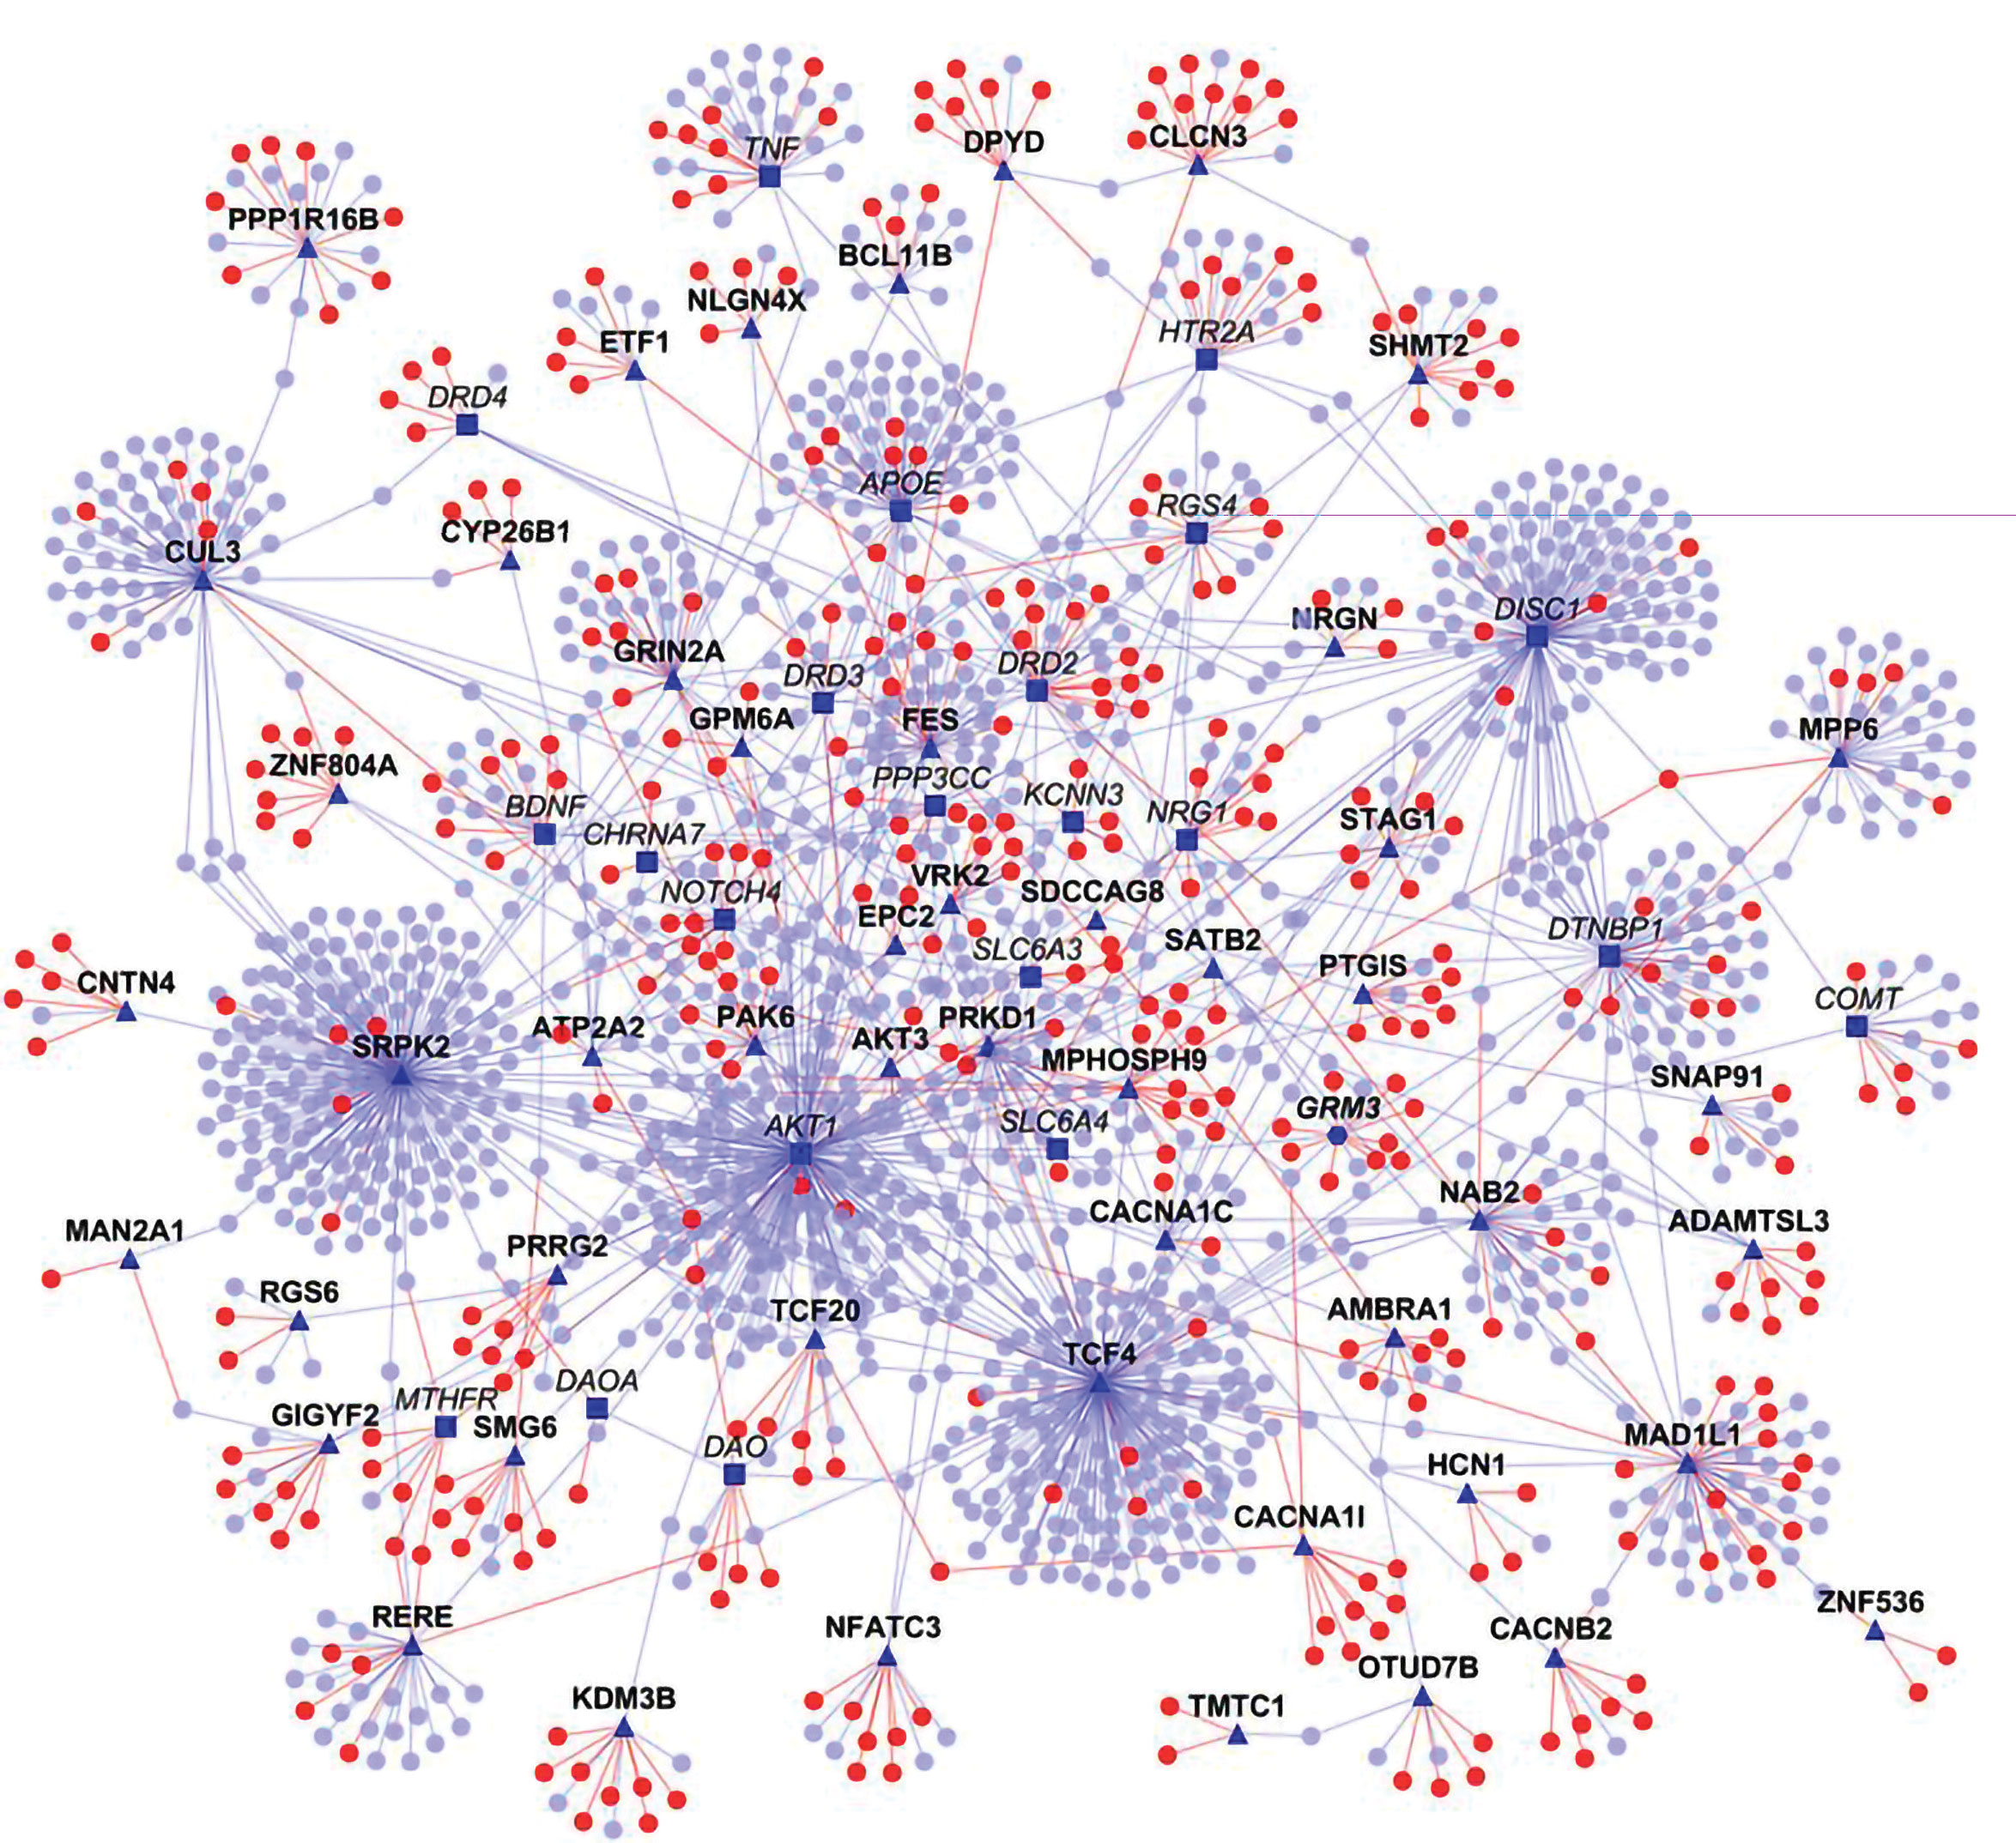
\includegraphics[width=0.4\textwidth,height=0.35\textheight, keepaspectratio]{figures/s2/protein_networks.jpg}};
        \node at (2.5,-3.7){Protein Interaction Networks};
    
        \node at (10.5,-1.9) {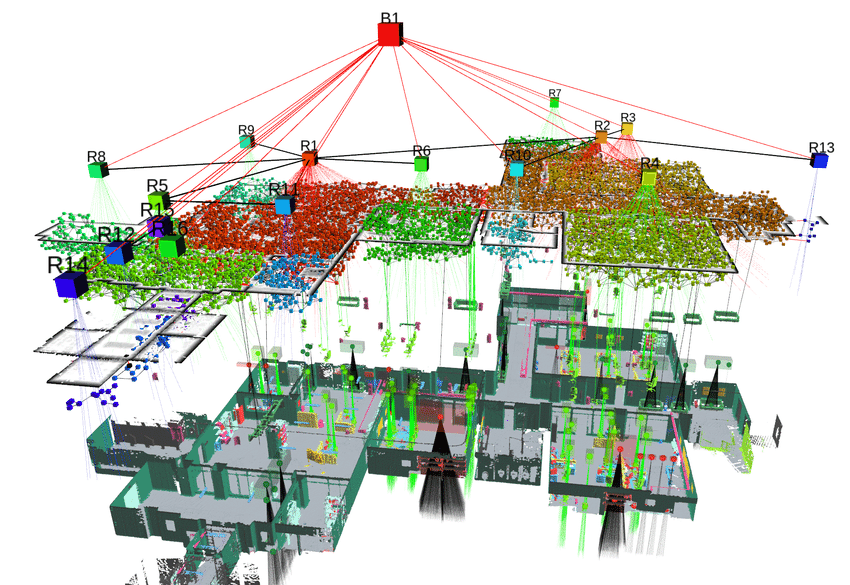
\includegraphics[width=0.4\textwidth,height=0.4\textheight, keepaspectratio]{figures/s2/scenegraphs.png}};
        \node at (10.5,-3.9){3D Scene Graphs};
    
        \node at (11.5,1.8) {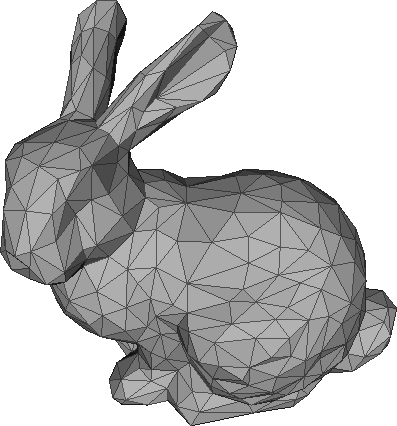
\includegraphics[width=0.38\textwidth,height=0.3\textheight, keepaspectratio]{figures/s2/bunny.png}};
        \node at (11.5,0.2){3D Shapes};
    \end{tikzpicture}
\end{frame}

\begin{frame}{Rethinking Convolutions: The Graph Way}
  \begin{minipage}{0.4\textwidth}
    \begin{itemize}
        \item Why are graphs useful?
        \item Why is it difficult to define convolution on graphs?
        \item What makes a neural network a graph neural network?
    \end{itemize}
  \end{minipage}%
  \hfill
  \begin{minipage}{0.55\textwidth}
    \centering
    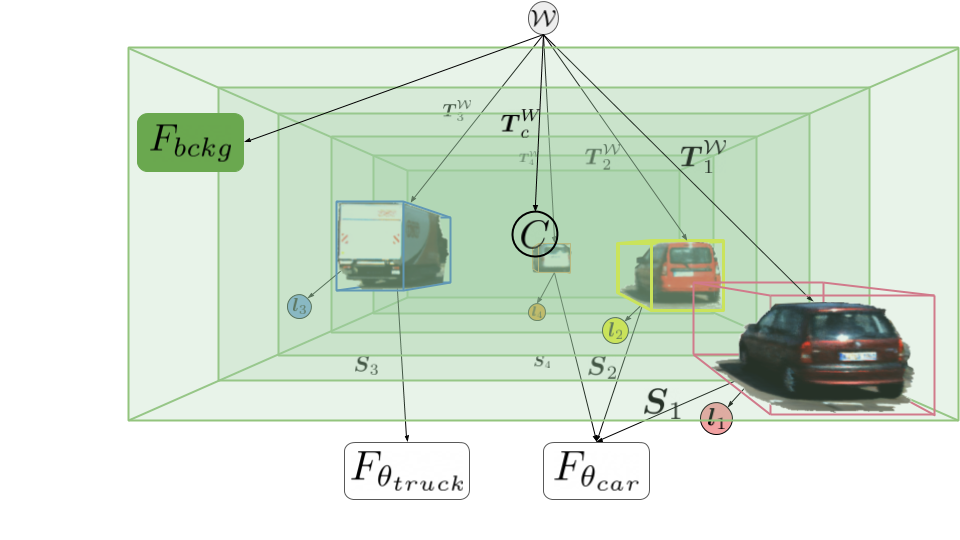
\includegraphics[width=\linewidth]{figures/scene_graph_perspective_small.png}
    \captionof*{figure}{\footnotesize \cite{ost2021neural}}
  \end{minipage}
\end{frame}


%------------------------------------------------

\begin{frame}[plain]
  \begin{tikzpicture}[remember picture, overlay]
    \node[opacity=0.35, at=(current page.center)] {
      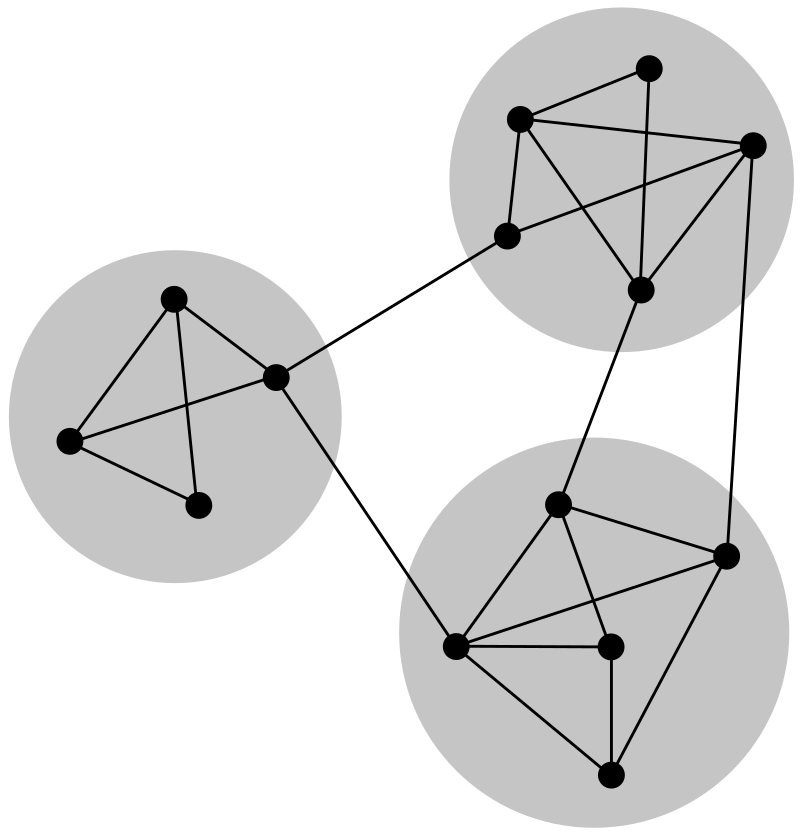
\includegraphics[width=0.5\paperwidth]{figures/Network_Community_Structure.svg.png}
    };
  \end{tikzpicture}

  \frametitle{Graphs Are What \textit{You} Make of Them}
  \begin{itemize}
    \item A graph $G$ is a collection of:
    \begin{itemize}
      \item \textbf{Nodes (vertices)} — the entities
      \item \textbf{Edges} — the relationships (directed or undirected)
    \end{itemize}

    \pause
    \item The graph structure often comes from your \textbf{domain knowledge or intuition}

    \pause
    \item You decide:
    \begin{itemize}
      \item Atoms $\leftrightarrow$ Molecules
      \item Users $\leftrightarrow$ Social Networks
      \item Cities $\leftrightarrow$ Transportation Systems
      \item Players $\leftrightarrow$ Team Sports
      \item Neurons $\leftrightarrow$ Brain Networks
      \item Objects $\leftrightarrow$ Physical Systems
      \item Pixels, Bounding Boxes $\leftrightarrow$ Images
    \end{itemize}

    \pause
    \item \textit{"In practice, you define what the nodes and edges represent."}
  \end{itemize}
\end{frame}

%------------------------------------------------
\section{Why are graphs useful?}
%------------------------------------------------

\begin{frame}{ Graphs as Alternative Data Representations}
    \begin{itemize}
        \item Provide alternative and flexible data representations.
        \item Many CV/ML tasks can benefit from viewing data as graphs rather than arrays or tensors.
        \item Graphs offer flexibility in capturing spatial and semantic relationships.
        \begin{itemize}
            \item Superpixel graphs in images (\cite{liang2016semantic})
            \item Human pose as a skeleton graph (\cite{yan2018spatial})
            \item Videos as graphs of moving objects (\cite{wang2018videos})
            \item Faces via facial landmark graphs (\cite{antonakos2015active})
        \end{itemize}
    \end{itemize}
    % \pause
    \begin{figure}
        \centering
        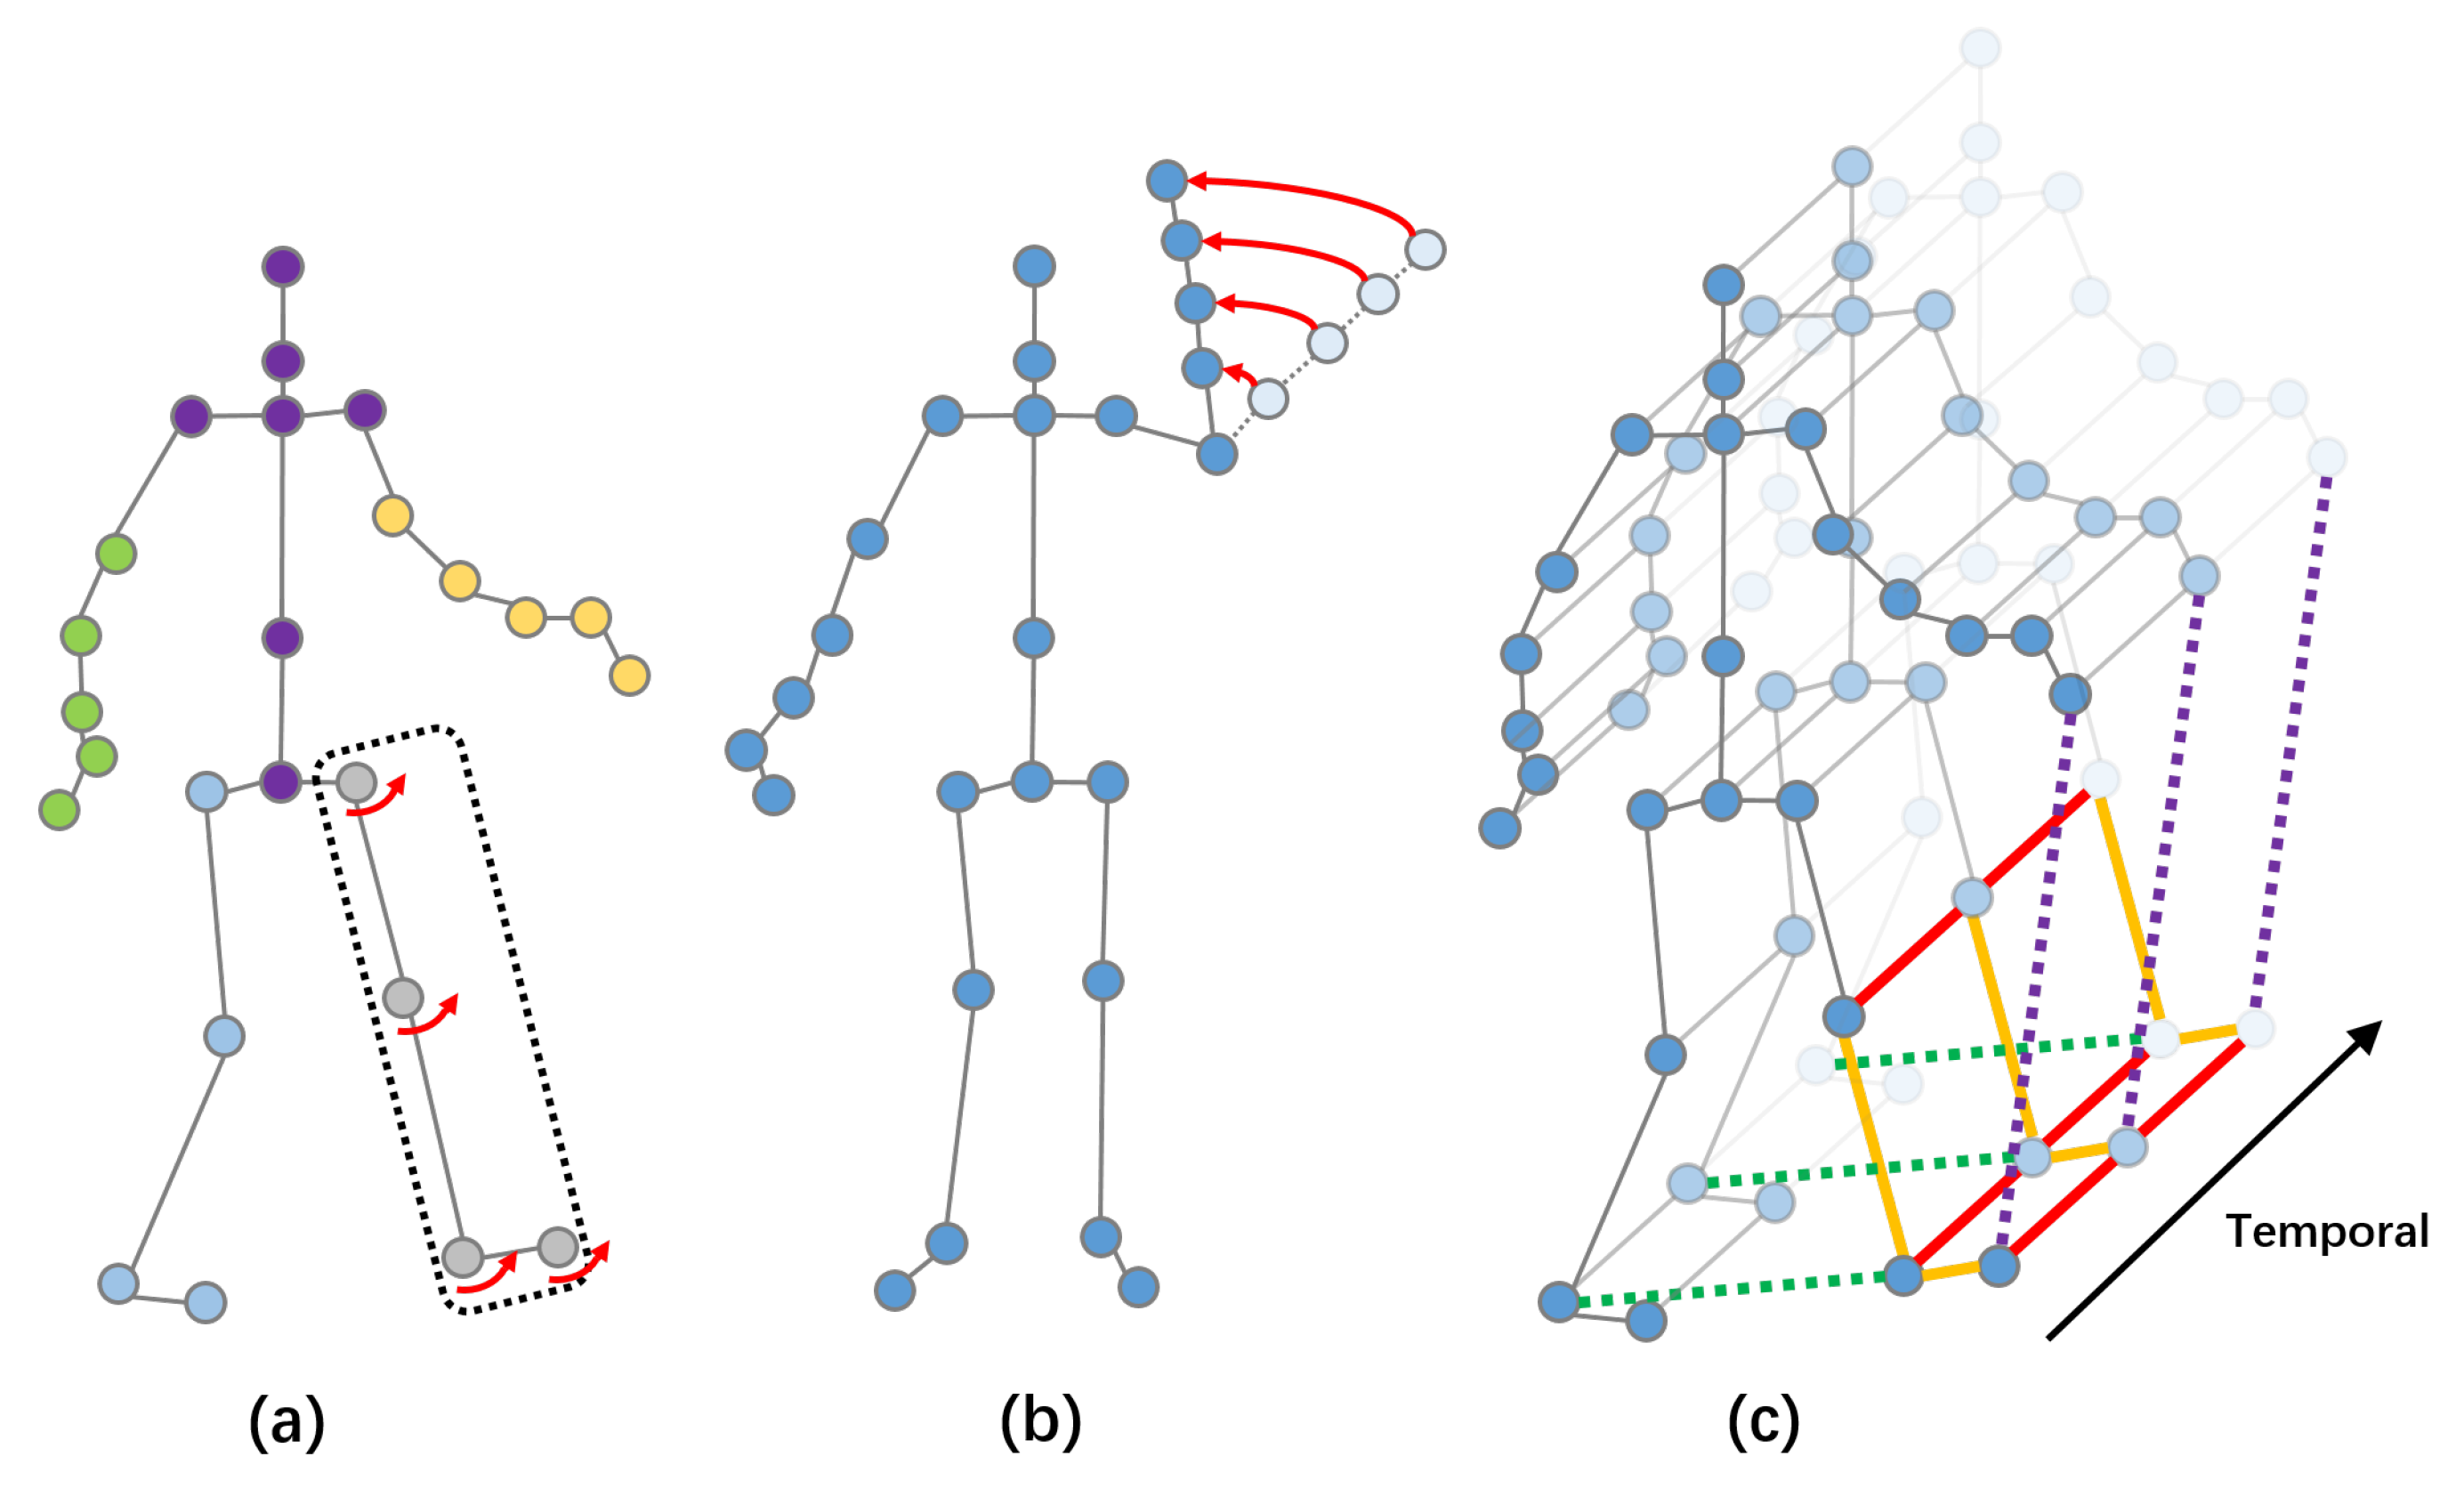
\includegraphics[width=0.49\linewidth]{figures/skeleton_graph.png}
        % \caption{Caption}
        % \label{fig:enter-label}
    \end{figure}
\end{frame}

\begin{frame}{Graphs are Natural for Many Learning Tasks}
    \begin{itemize}
        \item Many problems are naturally graph-structured:
        \begin{itemize}
            \item Molecule and social network classification (\cite{knyazev2018spectral})
            \item 3D mesh processing (\cite{fey2018splinecnn})
            \item Dynamic systems modeling (\cite{kipf2018neural})
            \item Visual scene graphs and reasoning (\cite{narasimhan2018out})
            \item Program synthesis and RL tasks (\cite{bapst2019structured})
        \end{itemize}
        \item GNNs empower learning from these rich relational structures.
    \end{itemize}
    % \pause
    \begin{figure}
        \centering
        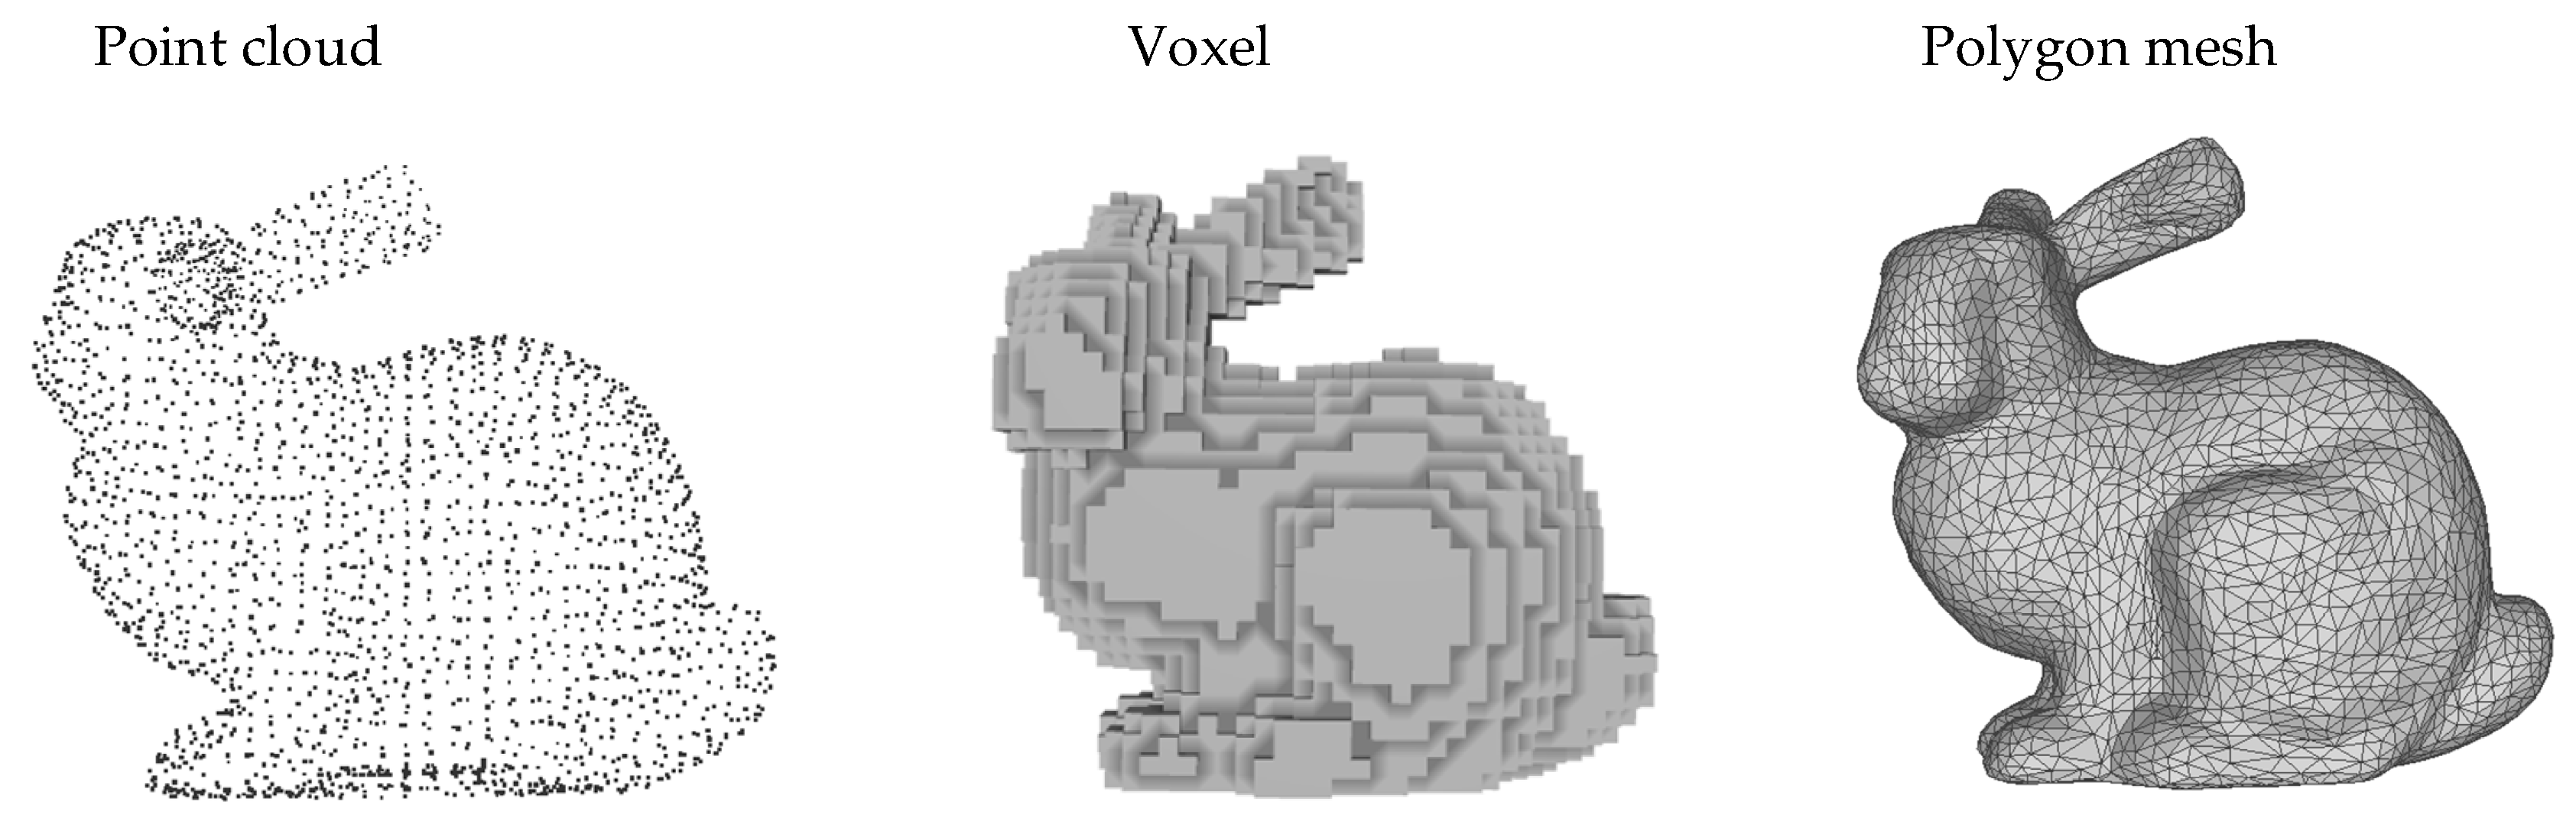
\includegraphics[width=0.5\linewidth]{figures/3d_mesh.png}
        % \caption{Caption}
        % \label{fig:enter-label}
    \end{figure}
\end{frame}


\begin{frame}{A Gateway to Solving Complex Real-World Problems}
    \begin{itemize}
        \item Enables tackling previously unsolvable real-world problems:
        \begin{itemize}
            \item Drug discovery (\cite{veselkov2019hyperfoods})
            \item Human brain connectivity (\cite{diez2018neurogenetic})
            \item Materials discovery for energy and environmental challenges (\cite{xie2019graph})
        \end{itemize}
    \end{itemize}

    % \pause
    
    \begin{figure}
        \centering
        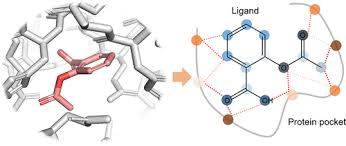
\includegraphics[width=0.5\linewidth]{figures/ligand.jpg}
        % \caption{Caption}
        % \label{fig:enter-label}
    \end{figure}
\end{frame}

%------------------------------------------------
\section{Why is it difficult to define convolution on graphs?}
%------------------------------------------------

\begin{frame}{Why is convolution useful?}
    \begin{figure}
        \centering
        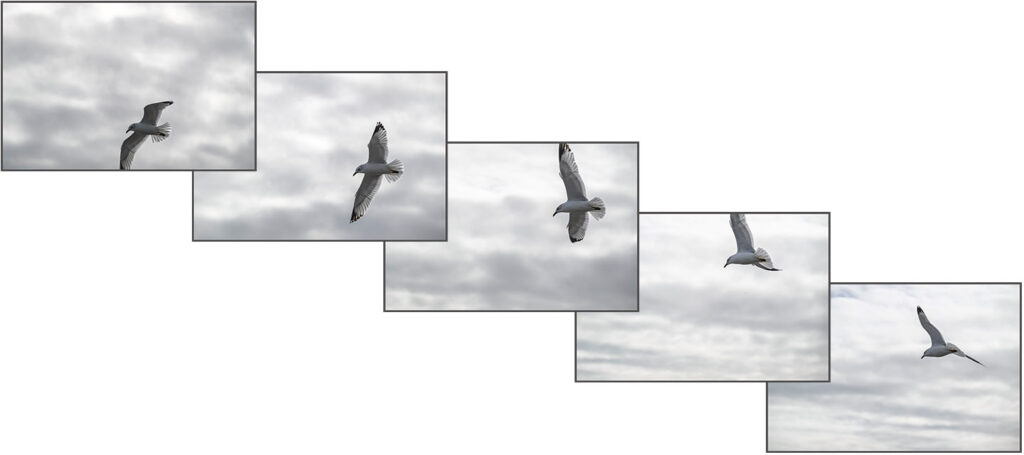
\includegraphics[width=0.5\linewidth]{figures/gull-5-shot-burst-1024x455.jpg}
        % \caption{Caption}
        % \label{fig:enter-label}
    \end{figure}
    \begin{itemize}
        \item CNNs exploit:
        \begin{itemize}
            \item Shift invariance
            \item Locality
            \item Compositionality (or hierarchy)
            \item Convolutional layers are parametric
        \end{itemize}
    \end{itemize}
\end{frame}

%------------------------------------------------

\begin{frame}{Convolution on Images in Terms of Graphs}
    \begin{figure}
        \centering
        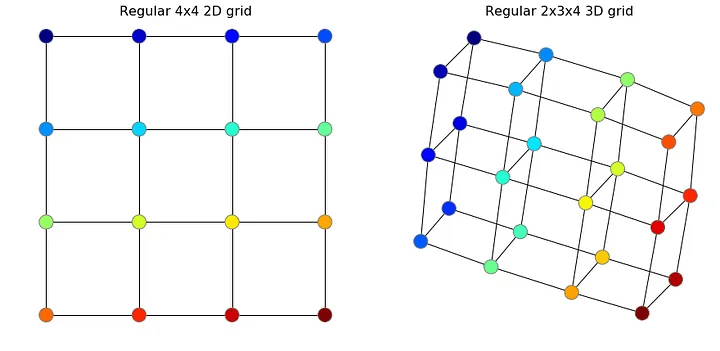
\includegraphics[width=0.5\linewidth]{figures/grid_graph.png}
        \caption*{Examples of regular 2D and 3D grids.}
    \end{figure}
    \begin{itemize}
        \item Let's apply conv filters on this
    \end{itemize}
\end{frame}

\begin{frame}{Convolution on Images in Terms of Graphs}
    \begin{figure}
        \centering
        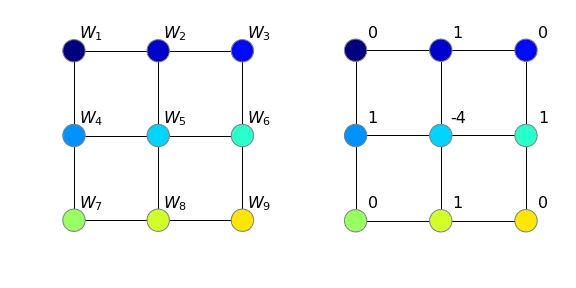
\includegraphics[width=0.5\linewidth]{figures/filter.png}
        \caption*{3×3 filter on a regular 2D grid with arbitrary weights w and an edge detector.}
    \end{figure}
    \begin{itemize}
        \item  We slide over all possible locations.
        \item We compute the dot product:
    $$W:X_1W_1+X_2W_2+...+X_9W_9$$
    \end{itemize}
\end{frame}

\begin{frame}{Convolution on Images in Terms of Graphs}
    \begin{figure}
        \centering
        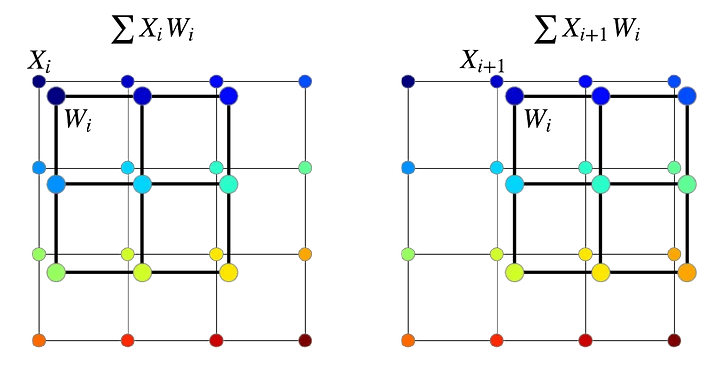
\includegraphics[width=0.5\linewidth]{figures/convolution.png}
        \caption*{2 steps of 2D convolution on a regular grid.}
    \end{figure}
    \begin{itemize}
        \item The dot product is an aggregator operator.
        \item It summarizes a 3×3 matrix to a single value.
        \item But is not permutation invariant. i.e.
        $$X_1W_1+X_2W@ \neq X_1W_2+X_2W_1$$
    \end{itemize}
\end{frame}

\begin{frame}{Convolution on Images in Terms of Graphs}
    \begin{figure}
        \centering
        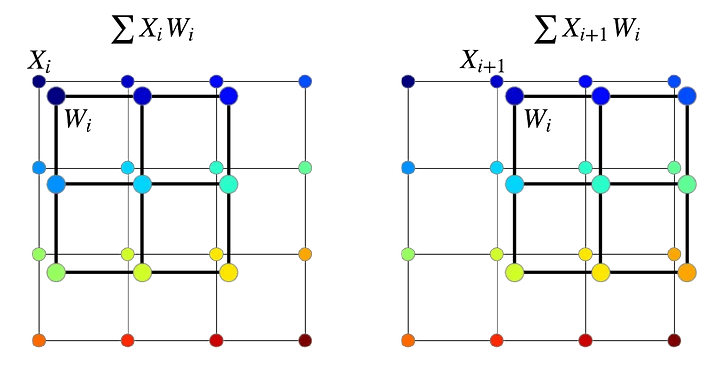
\includegraphics[width=0.5\linewidth]{figures/convolution.png}
        \caption*{2 steps of 2D convolution on a regular grid.}
    \end{figure}
    \begin{itemize}
        \item  In a regular grid, we always can match a node of the filter with a node of the grid.
        % \pause
        \item Let's see this in action on MNIST.
    \end{itemize}
\end{frame}

\begin{frame}{Convolution on Images in Terms of Graphs}
    \begin{figure}
        \centering
        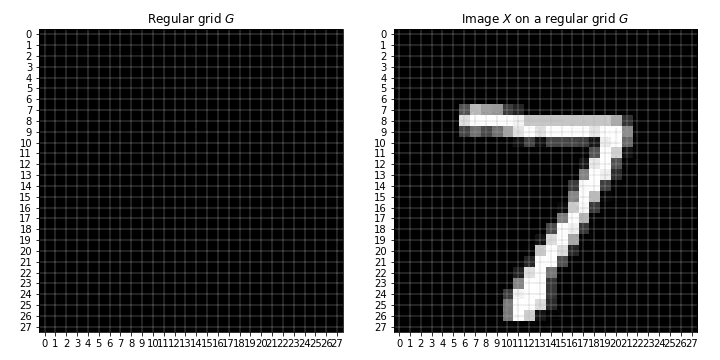
\includegraphics[width=0.5\linewidth]{figures/MNIST_2.png}
        \caption*{Regular 28×28 grid and an image on that grid.}
    \end{figure}
    \begin{itemize}
        \item Define a filter with arbitrary parameters and perform convolution.
    \end{itemize}
\end{frame}

\begin{frame}{Convolution on Images in Terms of Graphs}
    \begin{figure}
        \centering
        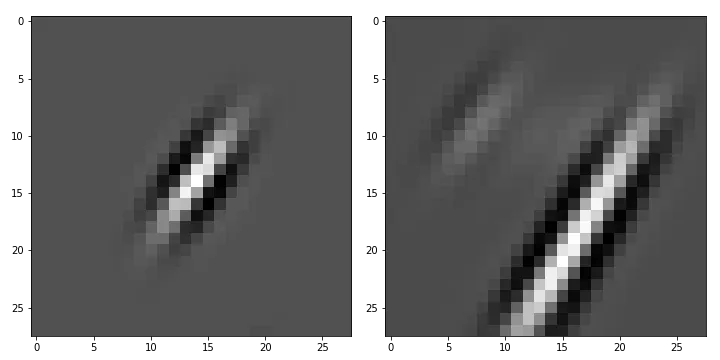
\includegraphics[width=0.5\linewidth]{figures/conv_out.png}
        \caption*{A 28×28 filter and the result of 2D convolution of this filter with the image of digit 7.}
    \end{figure}
    \begin{itemize}
    \item Can we generalize convolution to graphs?
    \end{itemize}
\end{frame}

\begin{frame}{Convolution on Images in Terms of Graphs}
    \begin{figure}
        \centering
        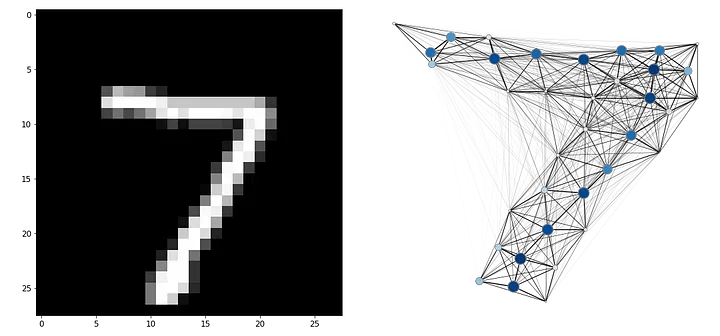
\includegraphics[width=0.5\linewidth]{figures/mnist7.png}
        \caption*{An image from the MNIST dataset and its graph representation.}
    \end{figure}
     \begin{itemize}
        \item Nodes in a graph form an unordered set.
        % \pause
        \item Any permutation of the node set does not change the graph.
        % \pause
        \item Therefore, the aggregator must be \textbf{permutation-invariant}.
        % \pause
        \item In graphs, there’s no consistent node order — unless you learn or enforce one.
    \end{itemize}
\end{frame}

\begin{frame}{Convolution on Images in Terms of Graphs}
    \begin{figure}
        \centering
        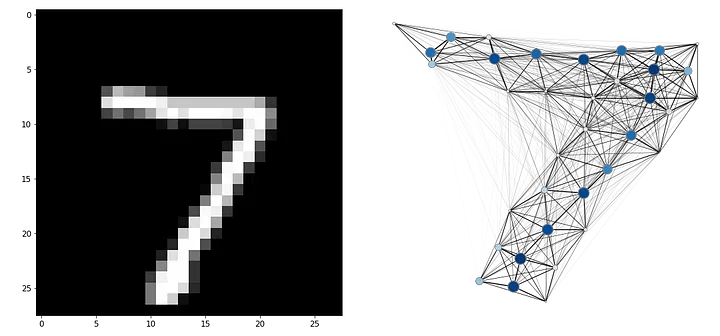
\includegraphics[width=0.35\linewidth]{figures/mnist7.png}
        \caption*{An image from the MNIST dataset and its graph representation.}
    \end{figure}
     \begin{itemize}
        \item Solution: Use permutation-invariant aggregators.
        \begin{itemize}
            \item \footfullcite{kipf2016semi}: Mean aggregation 
            \item \footfullcite{xu2018powerful}: Sum aggregation
            \item \footfullcite{hamilton2017inductive}: GraphSAGE
        \end{itemize}
    \end{itemize}
\end{frame}

\begin{frame}{Convolution on Images in Terms of Graphs}
    \begin{figure}
        \centering
        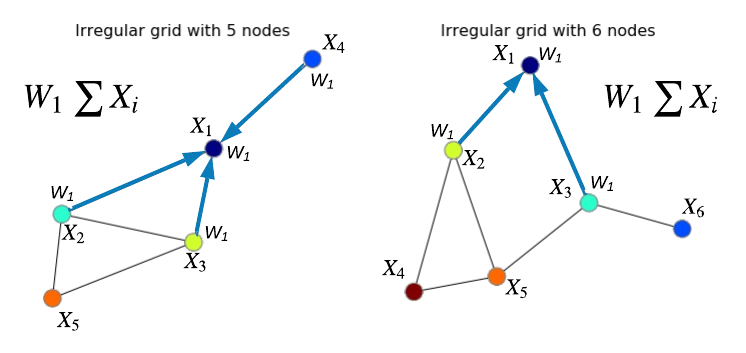
\includegraphics[width=0.5\linewidth]{figures/graph_conv.png}
        \caption*{Convolution on graphs of node features X with filter W centered at node 1 }
    \end{figure}

   \begin{itemize}
        \item Node 1: \( h_1 = (x_1 + x_2 + x_3 + x_4)W \)
        \item Node 2: \( h_2 = (x_1 + x_2 + x_3 + x_5)W \)
        \item Continue similarly for other nodes...
        
    \end{itemize}
\end{frame}

\begin{frame}{Convolution on Images in Terms of Graphs}
    \begin{figure}
        \centering
        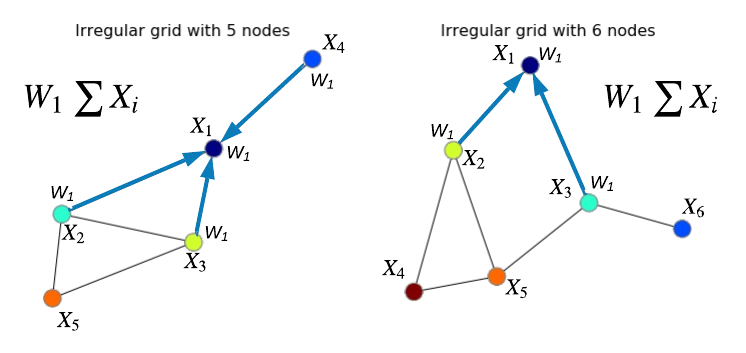
\includegraphics[width=0.5\linewidth]{figures/graph_conv.png}
        \caption*{Convolution on graphs of node features X with filter W centered at node 1 }
    \end{figure}

   \begin{itemize}
       
        \item Use the \textbf{same weight matrix \( W \)} for all nodes.
        \item Produces \textbf{new node features} enriched with neighbor information.
        \item The graph structure remains unchanged, only the node features are updated.
        \item \textbf{Stack multiple layers} to let information flow deeper into the graph.
    \end{itemize}
\end{frame}

%------------------------------------------------
\section{What makes a neural network a graph neural network?}
%------------------------------------------------

\begin{frame}{What makes a neural network a graph neural network?}
    \begin{itemize}
        \item In a vanilla neural network, the output of layer $l$ is:
      $$X^{(l+1)} = X^{(l)}W^{(l)} $$
        \item But this operation ignores graph structure — it's just applied row-wise.
        \item How do we transform this to a graph neural network?
        \pause
        \item  The core idea behind GNNs is aggregation over \textbf{neighbors} specified by \textit{you}.
    \end{itemize}
\end{frame}

\begin{frame}{What makes a neural network a graph neural network?}
    \begin{figure}
        \centering
        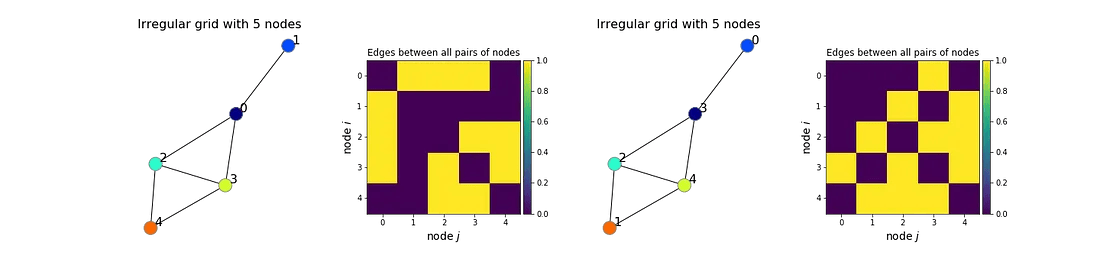
\includegraphics[width=0.75\linewidth]{figures/adjacency.png}
        \caption*{The order of nodes we defined in both cases is random, while the graph is still the same.}
    \end{figure}

    \begin{itemize}
        \item Adjacency matrix represents edges in matrix form.
        \item Each row/column in $A$ corresponds to a node.
        \item This encodes “who is connected to whom”.
        \item It is the prior/inductive bias we impose on our model.
    \end{itemize}
\end{frame}

\begin{frame}{What makes a neural network a graph neural network?}
    \begin{figure}
        \centering
        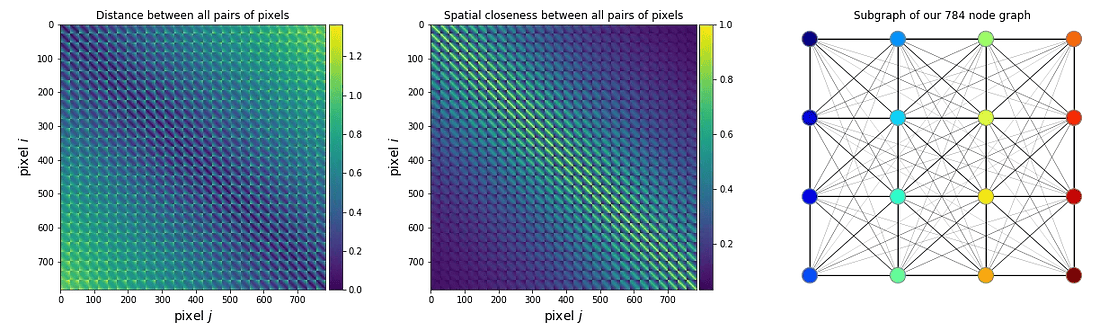
\includegraphics[width=0.75\linewidth]{figures/adj_mnist.png}
        \caption*{Adjacency matrix (NxN) in the form of distances and closeness between all pairs of nodes. A subgraph with 16 neighboring pixels corresponding to the adjacency matrix in the middle. }
    \end{figure}

    \begin{itemize}
        \item Instead of having just features $X$ we have a matrix $A$.
        \item But there is no canonical order of nodes that will be consistent across all other graphs in the dataset.
    \end{itemize}
\end{frame}

\begin{frame}{What makes a neural network a graph neural network?}
    \begin{figure}
        \centering
        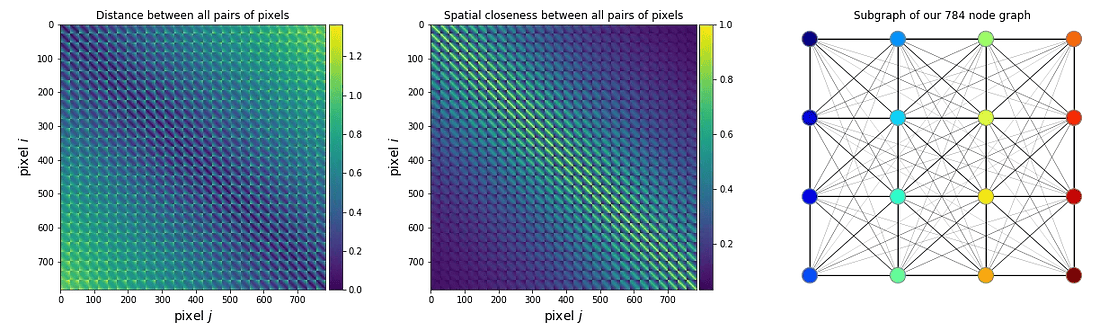
\includegraphics[width=0.75\linewidth]{figures/adj_mnist.png}
        \caption*{Adjacency matrix (NxN) in the form of distances and closeness between all pairs of nodes. A subgraph with 16 neighboring pixels corresponding to the adjacency matrix in the middle. }
    \end{figure}

    \begin{itemize}
        \item Regular MLPs assume the order of input features matters (like pixels in an image).
        \item In graphs, node order is arbitrary, so that assumption breaks.
        \item Using the adjacency matrix $A$ helps us do learning in a way that doesn't care about node order — and that's what Graph Neural Networks are built for.
    \end{itemize}
\end{frame}

\begin{frame}{Graph Neural Networks}
    \begin{itemize}
        \item We want to update the features of each node by combining info from its neighbors — this is \textbf{message passing}.
        \item Multiply the adjacency matrix with the feature matrix
        $$X^{(l+1)} = \mathcal{A}X^{(l)}W^{(l)}$$
        where $\mathcal{A}=\frac{A}{\sum_i A_i}$
        \item This is the core of a Graph Convolutional Network (GCN).
    \end{itemize}
\end{frame}

%------------------------------------------------
\begin{frame}{Other Visual Node representations}
    \begin{figure}
        \centering
        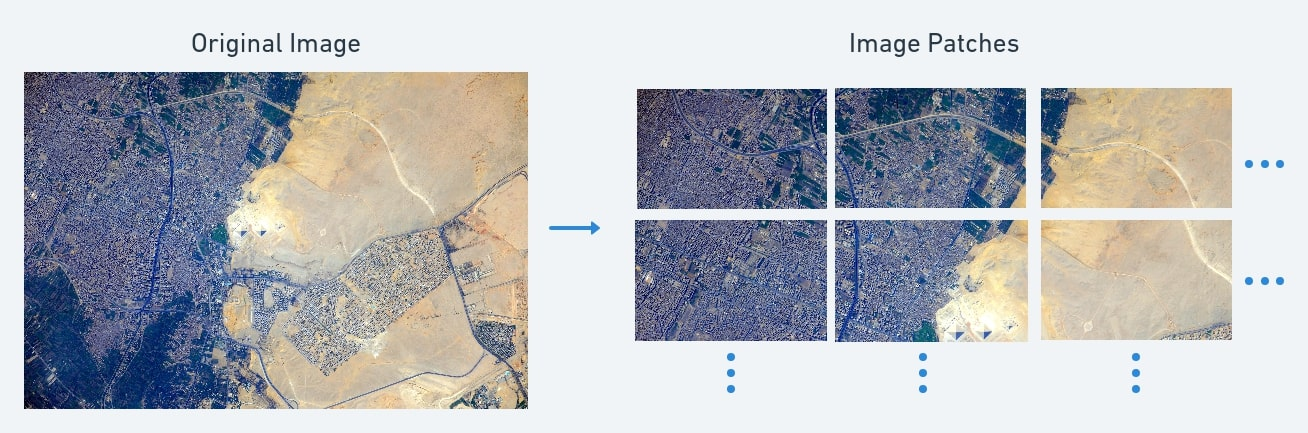
\includegraphics[width=0.5\linewidth]{figures/super_pixels.jpeg}
    \end{figure}
    \begin{itemize}
        \item Split an image into fixed-size patches and view as nodes.
        \item Parse images into semantic graphs of objects and relationships — enabling structured understanding for downstream tasks.
    \end{itemize}
    \footfullcite{li2019pastegan}
\end{frame}

\begin{frame}{Other Visual Node representations}
    \begin{figure}
        \centering
        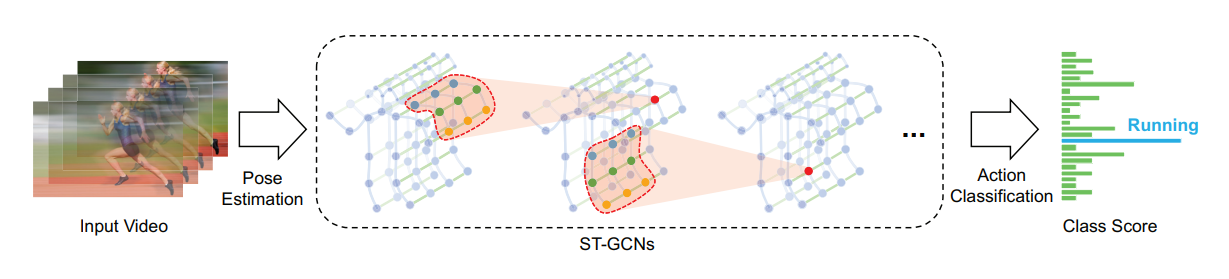
\includegraphics[width=0.85\linewidth]{figures/STGCN.png}
    \end{figure}
    \begin{itemize}
        \item Human joints linked by
skeletons naturally form a graph and learn human action patterns.
    \end{itemize}
    \footfullcite{yan2018spatial}
\end{frame}

\begin{frame}{Other Visual Node representations}
    \begin{figure}
        \centering
        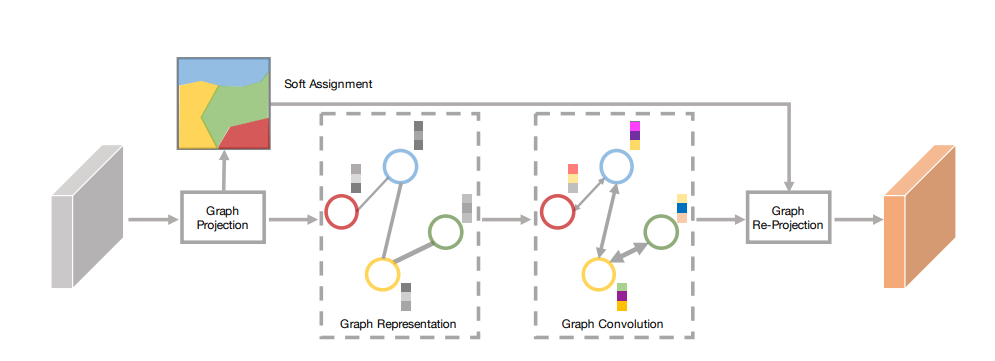
\includegraphics[width=0.7\linewidth]{figures/semantic_pixel.png}
    \end{figure}
    \begin{itemize}
        \item Assign pixels with similar features to the same vertex grouping pixels into coherent regions.
    \end{itemize}
    \footfullcite{li2018beyond}
\end{frame}

\begin{frame}{Other Visual Node representations}
    \begin{figure}
        \centering
        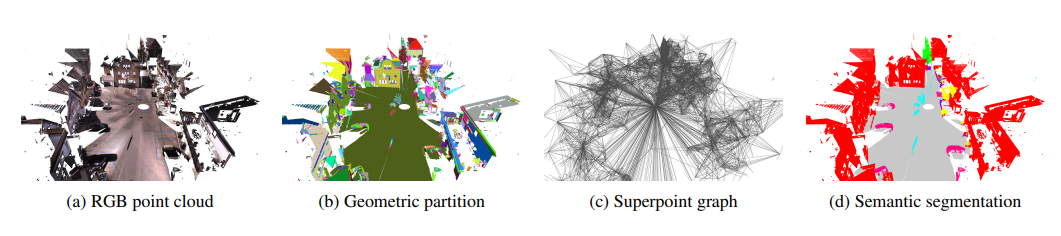
\includegraphics[width=0.85\linewidth]{figures/pt_cld.png}
    \end{figure}
    \begin{itemize}
        \item Aggregate k-nearest neighbors into superpoints (nodes), then use GCNs to model their relationships and understand the topology of the surrounding environment.
    \end{itemize}
    \footfullcite{landrieu2018large}
\end{frame}
%------------------------------------------------

\begin{frame}{Visual Edge Representation in GNNs}
    \begin{itemize}
        \item \textbf{Edges capture spatial and temporal relations} between visual elements (e.g., objects, regions, patches).
        % \pause
        \item \textbf{Spatial Edges:}
        \begin{itemize}
            \item Fixed using scene graphs or human skeletons (static).
            \item Learned dynamically via self-attention or fully-connected graphs.
        \end{itemize}
        % \pause
        \item \textbf{Temporal Edges:}
        \begin{itemize}
            \item Link nodes across frames using k-NN or semantic similarity.
            \item Dynamic methods like random walks (Markov chains) model evolving node relations.
        \end{itemize}
        % \pause
        \item GNNs (spectral/spatial) leverage these edges to understand images and video over space and time.
    \end{itemize}
\end{frame}

\begin{frame}{Visual Caption, QA}
    \begin{figure}
        \centering
        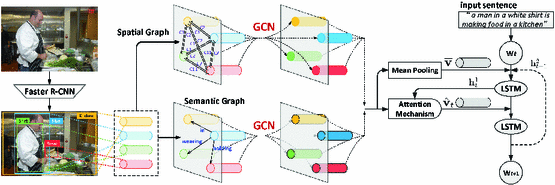
\includegraphics[width=0.85\linewidth]{figures/visual_caption.png}
    \end{figure}
    \begin{itemize}
        \item After detecting image regions a semantic/spatial graph is built where nodes are regions and edges capture relationships.
        \item The relation-aware features are passed through attention-based LSTM decoders to generate captions.
    \end{itemize}
    \footfullcite{yao2018exploring}
\end{frame}

%------------------------------------------------

\begin{frame}[allowframebreaks]{References}
    \footnotesize
    \printbibliography
\end{frame}

%------------------------------------------------

\begin{frame}
    \Huge{\centerline{\textbf{The End}}}
\end{frame}

%----------------------------------------------------------------------------------------

\end{document}